\documentclass{report}

\usepackage[top=1.5in,left=1.5in,bottom=1.5in,right=1.5in]{geometry}
\usepackage{amsmath}
\usepackage{bookmark}
\usepackage{listings} % for including nicely formatted code
\usepackage{array} % Included to solve invalid char in Tables declaration
\usepackage{graphicx} % to insert images
\graphicspath{{../pdf/}{/Users/rutviksayankar/Repos/ECE445_SP24/Paperwork/FinalReportLatexEnvironment/Images}} % setting up path for image storage

\usepackage{hyperref} % allows table of contents to be clickable to sections
\hypersetup{
    colorlinks,
    citecolor=blue,
    filecolor=blue,
    linkcolor=blue,
    urlcolor=blue
}

% Setting color formatting for Python code
\lstset{
    language=Python,
    frame=tb,
    basicstyle=\fontsize{8}{10}\ttfamily,
    keywordstyle=\color{blue},
    stringstyle=\color{red},
    commentstyle=\color{green},
    morecomment=[l][\color{magenta}]{\#},
}

% Setting color formatting for C code
\lstset{
    language=C,
    basicstyle=\fontsize{8}{10}\ttfamily,
    keywordstyle=\color{blue},
    stringstyle=\color{red},
    commentstyle=\color{magenta},
    morecomment=[l][\color{magenta}]{\#},
    frame=tb,
    numbers=left,
    % numberstyle=\tiny\color{gray},
    breaklines=true,
    showstringspaces=false,
}

% This section redefines the chapter headings, this allows us to remove the implicit "Chapter #" that comes before a provided chapter title.
\makeatletter
\def\@makechapterhead#1{%
  \vspace*{20\p@}%
  {\parindent \z@ \raggedright \normalfont
    \ifnum \c@secnumdepth >\m@ne
      %\if@mainmatter
        %\huge\bfseries \@chapapp\space \thechapter
        \Huge\bfseries \thechapter.\space%
        %\par\nobreak
        %\vskip 20\p@
      %\fi
    \fi
    \interlinepenalty\@M
    \Huge \bfseries #1\par\nobreak
    \vskip 40\p@
  }}
\makeatother

\title{ECE 445: Senior Design Project Laboratory \\ Final Report \\ Oxygen Delivery Robot} % Sets article title

\author {
    \textbf{Team 27} \\ 
    \textit{Sayankar, Rutvik}\\
    \textit{rutviks2@illinois.edu} \\
    \hfill \\ 
    \textit{Dunican, Aidan}\\
    \textit{dunican2@illinois.edu} \\
    \hfill \\ 
    \textit{Kalyniouk, Nazar}\\
    \textit{nazark2@illinois.edu} \\
    \hfill \\ 
    \textbf{Teaching Assistant} \\ 
    \textit{Subramaniam, Selva} \\
    \textit{ss170@illinois.edu} 
} 
\date{\today} % Sets date for date compiled

% The preamble ends with the command \begin{document}
\begin{document}
    \maketitle % creates title using information in preamble (title, author, date)

    \begin{abstract}
        Mobile oxygen delivery is a mostly untapped market for users both elderly and young. This report details a prototype design for a mobile oxygen delivery robot. We utilize a three wheeled omni-directional drivetrain, ultra wideband triangulation, computer vision, and a simple Roomba style bumper system. We remove ourselves from the context of dealing with oxygen related tubing as swivel solutions already exist and focus on the issue of creating a robot that can autonomously and efficiently move an oxygen tank around in an indoor space.
    \end{abstract}
    
    \pagebreak
    \tableofcontents % creates table of contents
    \pagebreak

    \chapter{Introduction}
    \section{Project Overview}
    Children's interstitial and diffuse lung disease (ChILD) is a collection of diseases or disorders. These diseases cause a thickening of the interstitium (the tissue that extends throughout the lungs) due to scarring, inflammation, or fluid buildup \cite{ChILD-2022}. This eventually affects a patient’s ability to breathe and distribute enough oxygen to the blood. Numerous children experience the impact of this situation, requiring supplemental oxygen for their daily activities. It hampers the mobility and freedom of young children, diminishing their growth and confidence. Moreover, parents face an increased burden, not only caring for their child but also having to be directly involved in managing the oxygen tank as their child moves around.

    Given the absence of relevant solutions in the current market, our project aims to ease the challenges faced by parents and provide young children the freedom to explore their surroundings without worry. As a proof of concept for an affordable solution, we propose a three wheeled omni-directional mobile robot capable of supporting a filled M-6 oxygen tank. We plan to implement two localization subsystems to ensure redundancy and enhance child safety. The first subsystem utilizes Ultra-Wideband (UWB) transceivers for triangulating the child's location relative to the robot in indoor environments, this is similar to how Apple AirTags triangulate their location relative to an iPhone \cite{airtag_uwb} (although AirTags use a combination of UWB and Bluetooth triangulation \cite{airtag_ble}). The second subsystem makes use of a desktop web camera which streams video to a Raspberry Pi where it will leverage open-source object tracking libraries to improve our directional accuracy in tracking a child. The final subsystems will focus on close range object detection.

    \newpage

    \section{Block Diagram}
    \begin{figure}[ht!]
      \centering
      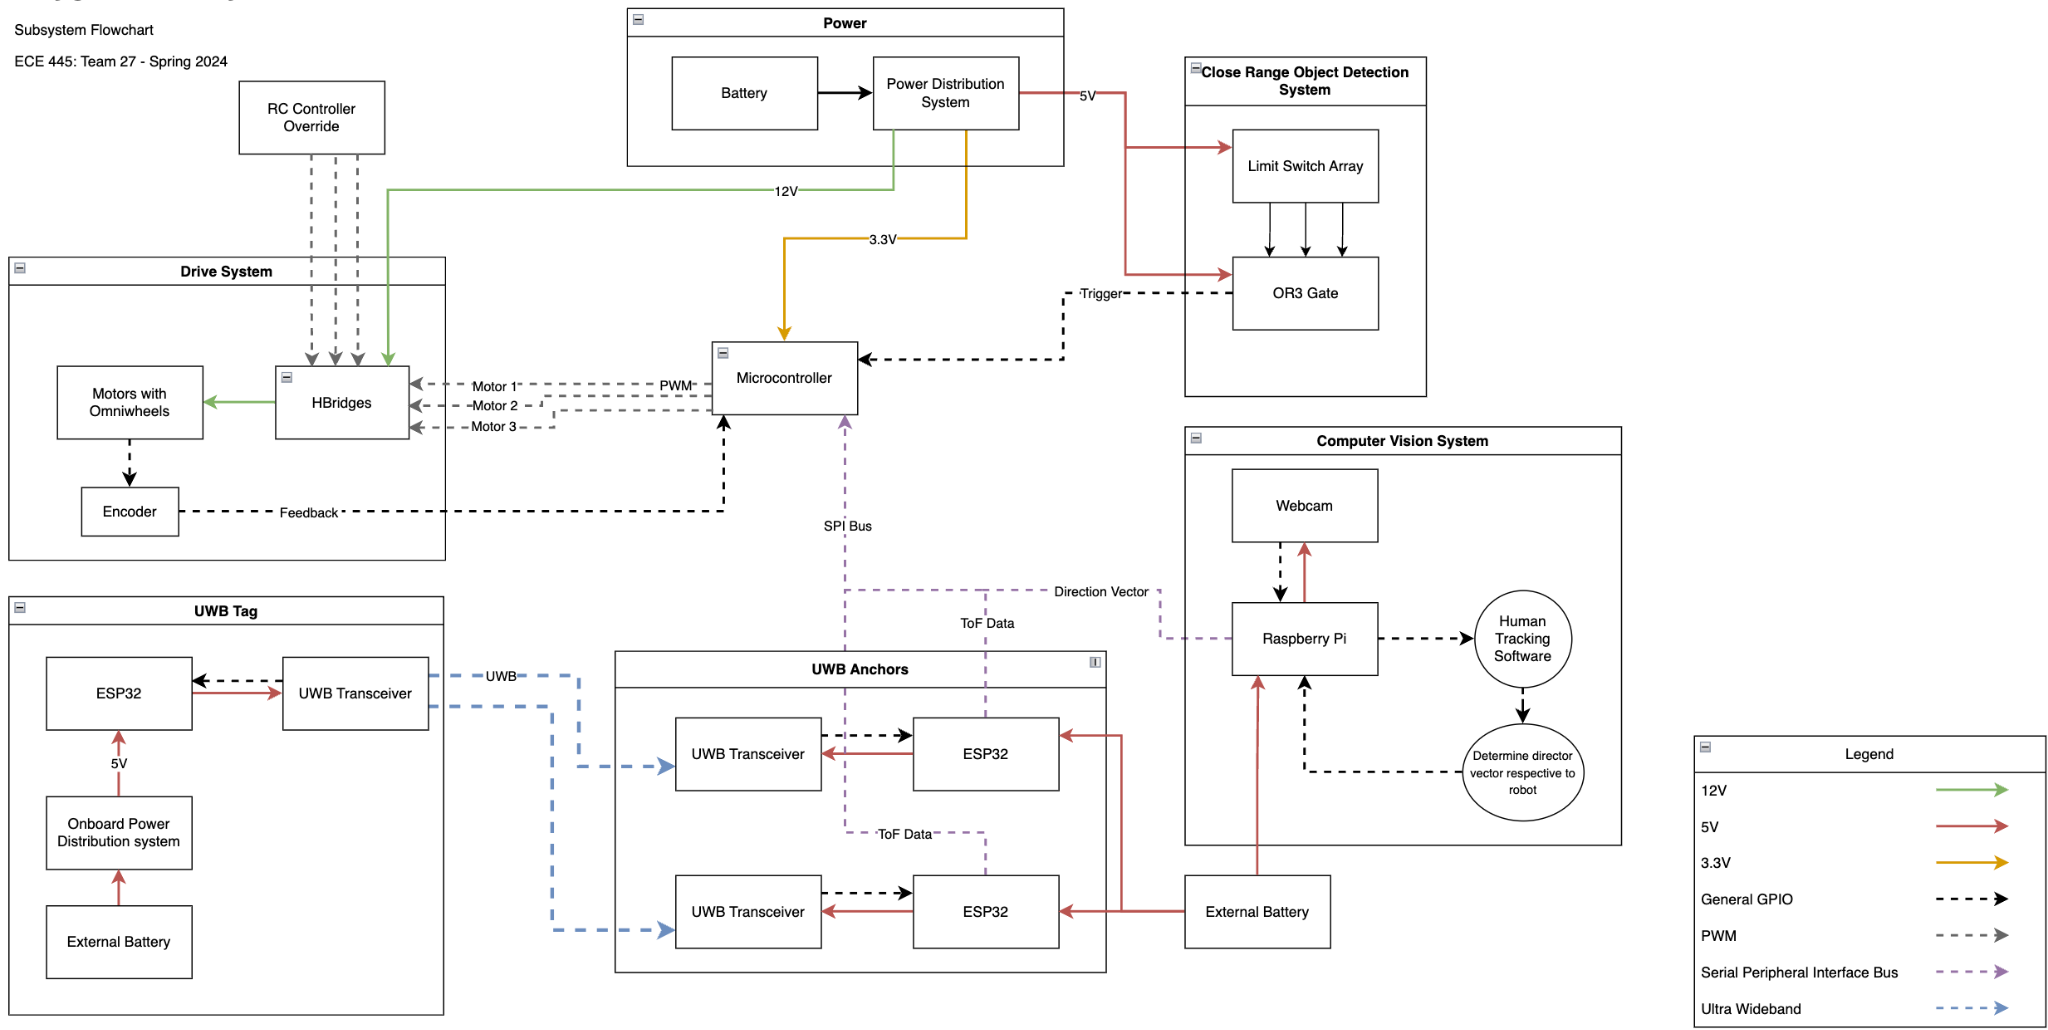
\includegraphics[width=1.2\textwidth]{Images/BlockDiagram.png}
      \caption{High Level Block Diagram}
      \label{fig:BlockDiagram}
  \end{figure}

    \subsection{Omniwheel Drivetrain System}
    We utilize a three wheeled omni-directional wheel drive train. In software we make use of simple matrix multiplication (detailed in section \ref{sec:Omniwheel-InverseKinematics}) to derive individual wheel speeds given that we know where we want to go in Cartesian space.

    \subsection{Ultra-Wideband Triangulation System}
    This system makes use of UWB transceivers in order to triangulate location in an indoor space with high accuracy. The goal was to be able to locate the user in an indoor environment where there maybe be interference with other bluetooth or wifi signals. 
    
    \subsection{Close Range Object Detection System}
    The Close Range Object Detection subsystem makes use of limit switches with bumpers attached to them arranged in a ring around the robot that will detect when it encounters an object in its path. The goal of this system is to halt the robot and any further movement when a limit switch is pressed. This enhances the safety of the robot, particularly in environments with children. With the expectation that the robot will be utilized inside spaces such as a living room which might have toys scattered around due to younger children being present. To limit the scope of the project we want the robot to simply stop movement upon collision with any object in it's path and have either the user or a someone supervising come in and clear the area before the robot is to be used again.
    
    \subsection{Computer Vision System}
    The Computer Vision subsystem was incorporated into our design to ensure redundancy and robustness. By having a sensor fusion between this and the UWB subsystem, we can ensure that the robot follows the child as desired and add an extra layer of redundancy and safety to our design. The performance requirements of this subsystem are that this subsystem will initiate a corrective measure to the STM32 microcontroller if the child deviates too far from the center of the input frame. Specifically, this system focuses on the degrees away from the center the user currently is. Between the start of this design and the end, nothing was changed in the block level of this subsystem.
    
    \subsection{Control System}
    This system is purely regarding how the STM32 microcontroller interacts and controls all our peripheral devices.
    
    \subsection{Power System}
    The power system of our robot was designed to take a 12V input and regulate it down to the 5V and 3.3V rails that will be used by all devices on our PCB. Specifically, for our 3.3V rail we needed to ensure a clean supply as it would be powering our STM32 microcontroller, which will be generating all of our PWM signals and reading a lot of timer related signals for which a clean 3.3V is preferred.


    \chapter{Design}
    \section{Design Procedure}

    \subsection{Omniwheel Drivetrain System}
    \label{sec:Omniwheel-DesignProcedure}

    We utilize a three wheeled omni-directional wheel drive train. Chosen mainly due to the cost benefit over a similar four wheeled drive train. This type of system is susceptible to drift in the form of yaw, therefore we made sure to include feedback from encoders back into our STM32 microcontroller to allow for drift compensation.

    \subsection{Ultra-Wideband Triangulation System}
    Our initial design discussion was regarding the type of wireless indoor localization we want to design. Immediately, two types of communication came to mind: UWB and BLE. Ultimately, we chose UWB over BLE due to the following benefits:

    \begin{itemize}
      \item Data transmission: UWB can transmit more data than Bluetooth Low Energy
      \item Accuracy: UWB can more accurately measure distance and determine position because it uses wideband radio waves and higher frequency bands
      \item Interference resistance: UWB is less likely to be affected by interference and obstructions
    \end{itemize}

    \subsubsection{Localization Algorithms} 
    To break it down simply, our goal was to find out the location of a user relative to our robot. We assume the user and robot will be in a valid location in real world space, and therefore can just focus on the user's location relative to our robot.

    To localize the user, we need to create a triangle of known lengths with vertices defined by the UWB transceivers. To obtain the lengths of each side we need to perform some ranging between the tag transceiver (the transceiver which the user will have) and the anchor transceivers (which are mounted onto the robot). With the anchors being a set 18" apart (the minimum as required by the DW3000 ICs we were using), we only needed the remaining two sides of our triangle.

    There are two ways to range between UWB transceivers. The first is to use Time of Flight (ToF). ToF is a positioning method based on two-way ranging. That means the tag needs to send and receive signals from the anchor several times and then the flight time of the signal between the anchor and the tag can be measured, because radio waves travel at the speed of light, we can calculate the distance between the tag and each anchor given that we know how long it took for a signal to travel between them. Secondly, Time Difference of Arrival (TDoA) is localization based on comparing the time difference between signals and each anchor and this technique requires an accurate time synchronization function. When using the TDoA method, the UWB tag will send out a poll message, and all the nearby UWB anchors will receive it and record the arrival time. Because the location of anchors is different, they will not receive the message at the same time. We can use these time differences to determine the tag’s location.

    Implementing an accurate time synchronization function between all of our transceivers increases the complexity of the project ten-fold therefore we decided to use a ToF based ranging method to calculate the distance between each anchor and the tag device.
    
    \subsection{Close Range Object Detection System}

    This system is the simplest but definitely required some debate in terms of how we wanted it implemented. We debated between two main types of detection: simple limit switches or ultrasonic sensors. Limit switches don't require explanation, you activate a switch and a signal goes high. The only struggle here would be finding a limit switch that would be suitable for our needs. The alternative was ultrasonic detection which would have required us to use a much larger number of sensors and which would have been much more sensitive. The reason we decided to use limit switches was that they would only stop the robot when an object collides with it. In addition, limit switches allow us to make a 360-degree bumper for the robot with only 3 switches, which would fill in the gap between each wheel. To design the subsystem we decided to go with the 3 Honeywell 101SN11 limit switches as they were the best available limit switch in the ECE Self-service center (put simply, it was the only limit switch that could take any sort of impact without damage). One of the major issues we had when designing this subsystem was how to get the Honeywell limit switches to work. Seeing as these limit switches have since been discontinued, finding proper documentation on them proved to be difficult. We discovered that the output to the limit switches needed a 10k pull-up resistor in order to drive the output high when the limit switch is inactive. This was all thanks to a helpful ebay seller who provided a simple explanation on the function of some old limit switches he was selling (\url{www.ebay.com/itm/333999755279 }).
    
    \subsection{Computer Vision System}
    Alternate approaches to incorporating person detection besides using a Haar cascade which we ultimately chose are as follows.
    
    \begin{itemize}
      \item Histogram of Oriented Gradients (HOG)
      \item You Only Look Once (YOLO)
      \item Single Shot MultiBox Detector (SSD)
    \end{itemize}
    
    Haar cascade was chosen for our final implementation as it is simpler to implement than conventional deep-learning models. It contains pre-trained full body models, a large stepping stone which would be required for our project. For the Haar cascade algorithm, a pre-trained model that detects full bodies is used. Once the body is detected, a bounding box is drawn around the body. The center point of this box and the center point of the screen are compared and this determines how far off the center the body is.
    
    \subsection{Control System}

    The details of the control system during design were fairly simple. It mainly consisted of choosing a microcontroller and deciding what pins to assign where. We were limited by what was provided by the ECE supply center, we decided to go with the F103 line of STM32 chips as we believed it had the perfect amount of GPIO and timer pins required for our robot. Our final pin assignments are shown in figure \ref{fig:STM32Pinout}.
    \\
    \\
    We required individual timers for the following:
    \begin{itemize}
      \item PWM output to motors (can all be synchronized therefore only need one timer)
      \item Motor 1 Encoder feedback
      \item Motor 2 Encoder feedback
      \item Motor 3 Encoder feedback
    \end{itemize}
We required GPIO for the following:

    \begin{itemize}
      \item Limit switch bumper input
      \item USB lines
      \item SPI bus
      \item Chip select for 3 peripherals on the SPI bus
      \item High Speed External Crystal Oscillator input and output.
      \item Programmer pins
    \end{itemize}
    
    \subsection{Power System}

    In our initial power design we had four requirements:

    \begin{itemize}
      \item Supply a max of $9~A$ at $12~V$ per motor therefore $27~A$ at $12~V$
      \item Supply $5~V$ to supply around $3.5~A$ line to power items like a Raspberry Pi running computer vision software, and two ESP32 boards that power the UWB transceiver anchors on the robot, and some other miscellaneous 5V powered ICs throughout our PCB.
      \item Supply $3.3~V$ at $< 80~mA$ for our STM32.
    \end{itemize}

    We initially began with separate buck converters for each of our power rails. This original design took up lots of space on our PCB and was unnecessary as we only needed one $5~V$ line rated for higher current. After realizing that our selection of ESP32 boards and Raspberry Pi's do not have the option of power delivery through GPIO pins, we decided to use an external battery pack to supply them power. But we opted to leave our higher current buck converter in the design to leave headroom for the possibility of delivering power to our Raspberry Pi and two ESP32 boards in the future. This led us to designing our final power system which consisted of a $12~V$ to $5~V$ buck converter rated for up to $6~A$. This was followed with a $5~V$ to $3.3~V$ LDO to supply the power to our $3.3~V$ line. The reason we opted to go with an LDO for the 3.3v was because it was supplying power to the microcontroller which due to its sensitivity needed to be at a stable $3.3~V$ ideally without much noise. By opting to go with an LDO we were able to lower the noise floor and improve the line regulation of the supply going to the STM32 and hopefully improve the analog performance of our microcontroller.

    To further ensure the performance of the our analog pins in our microcontroller we decided to make use a ferrite bead which suppresses high-frequency electronic noise in electronic circuits. Ferrite beads employ high-frequency current dissipation in a ferrite ceramic to build high-frequency noise suppression devices.

    \section{Design Details}

    \subsection{Omniwheel Drivetrain System}
    \subsubsection{Inverse Kinematics of the OWB}
    \label{sec:Omniwheel-InverseKinematics}
    In a three-wheeled omni-wheel robot, the three wheels are arranged in a triangular pattern, with one wheel at the front and two wheels at the back. Each wheel has several small omni-directional wheels arranged in a circular pattern, which allows the robot to move in any direction.
    
    To move the robot, each wheel is driven independently using a motor. By varying the speed and direction of each wheel, the robot can move in any direction and rotate around its center point.
    
    The kinematics of a three-wheeled omni-wheel robot can be modeled mathematically the below equations \cite{riky2021omnidirectional} which relate the robot's linear and angular velocities to the speed and direction of each wheel.
    
    We first define for each wheel a direction of rotation $V_i$, and the resulting movement effected in the x and y axes, $V_ix$ and $V_iy$ as shown below.

    Knowing the angle of each wheel from the vertical axis, we can compute the x and y components created by the rotation of each wheel. By summing these components together, we can get the effective motion of the robot in the x, y and yaw axes.
    
    \[
    \begin{pmatrix}
    V_x \\
    V_y \\
    \omega
    \end{pmatrix}
    =
    \begin{pmatrix}
    1 & - \frac{1}{2} & -\frac{1}{2} \\
    0 & -\frac{\sqrt{3}}{2} & \frac{\sqrt{3}}{2} \\
    1 & 1 & 1
    \end{pmatrix}
    \begin{pmatrix}
    V_1 \\
    V_2 \\
    V_3
    \end{pmatrix}
    \]
        
    $V_{x}$ and $V_{y}$ are the desired linear velocities in the x and y directions, respectively, and omega is the desired angular velocity. $V_{1}$, $V_{2}$, and $V_{3}$ are the velocities of the three wheels, and L is the distance between the robot's center of mass and the wheel axes.

    \[
    \begin{pmatrix}
    V_1 \\
    V_2 \\
    V_3
    \end{pmatrix}
    =
    \begin{pmatrix}
    1 & - \frac{1}{2} & -\frac{1}{2} \\
    0 & -\frac{\sqrt{3}}{2} & \frac{\sqrt{3}}{2} \\
    1 & 1 & 1
    \end{pmatrix}^{-1}
    \begin{pmatrix}
    V_x \\
    V_y \\
    \omega
    \end{pmatrix}
    \]

    By taking the inverse of our 3x3 component coefficient matrix above, we can solve for our individual motor speeds $V_1$, $V_2$ and $V_3$, given the desired motion in terms of $V_x$, $V_y$, and $w$.

    \subsection{RC Control}
    For drivetrain testing and part of our demo we used an RC controller. We made use of a Flysky FS-i6 6CH 2.4GHz Radio System RC Transmitter Controller with FS-iA6 Receiver (\ref{fig:RCController}). While the receiver supports up to six channels, the OWB only needs three channels. 

    The OWB can move forward and backward like a normal RC car. This motion is represented by $V_y$, and is mapped to CH1 on the transmitter. While a normal RC car needs a $V_y$ component to turn left or right, the OWB can "yaw" on the spot. This is represented by $w$, and is mapped to CH3 on the transmitter. The final unique motion the OWB can execute is a "drift" toward the left or right. This motion is represented by $V_x$ and is mapped to CH2 on the transmitter.

    Thus, using these three channels, the operator can define the robot's desired $V_x$, $V_y$, and $w$. These desired motion vectors are then fed to our inverse kinematics algorithm, which breaks down our desired motion into an individual wheel speed and direction for each motor.

    \subsection{Ultra-Wideband Triangulation System}

    The UWB triangulation utilizing double sided two way ranging between the tag device which will be attached to the user. This tag will performing this ranging calculation with each tag device, therefore deriving the lengths of each side of our localization triangle.

    \subsubsection{Symmetrical double-sided two-way ranging}
    Symmetrical double-sided two-way ranging (SDS-TWR) is a ranging method that uses two delays that naturally occur in signal transmission to determine the range between two stations \cite{IEEE_802}.

    \subsubsection{Signal Propagation Delay}
    When a test packet is transmitted from station A to station B, the propagation delay can be calculated. As the packet travels through space, the difference in time is calculated from when it's sent from the transmitter to the receiver. This time delay is known as the signal propagation delay.

    \subsubsection{Processing Delay}
    Following the transmission between station A and station B, station A waits for an acknowledgement from station B. Once station A takes a known amount of time to process the test packet, it generates an acknowledgement and prepares it for transmission. The time it requires to process the acknowledged message is referred to as the processing delay.

    \subsubsection{Range Calculation}
    The signal propagation delay and the processing delay are encapsulated in the acknowledgment sent back to station A. On this acknowledgment, station A computes another signal propagation delay. These three values are then used by the algorithm to calculate the range between station A and station B.

    \subsubsection{Verifying Range Calculation}
    To verify the accuracy of the previous range calculation, station B sends a test packet to station A and station A sends an acknowledgement to station B once it receives the signal. By repeating this procedure, the two range values are determined and an average can be calculated to verify the accuracy of the distance measurement between these two stations

    \subsection{Close Range Object Detection System}
    Once the Honeywell 101SN11 limit switch is pressed it drives the output voltage low. This signal is pulled high with a $10~k \Omega$ resistor (refer to figure \ref{fig:limitswitchcircuit}). Then fed directly to the CD74HC00N four channel two input NAND gate in order to invert the signal to high when the switch is pressed. From there the 3 inverted limit switch signals are passed on to a 3 input OR gate which combines the inputs into one single output, which is high when any limit switch is pressed. Next the output is passed to the one of the STM32's FT ($5~V$ tolerant) pins and which triggers an interrupt that will stop the PWM signals that drive the motors from being generated. This in turn halts the motors placing the robot in an idle state until the limit switch is unpressed and the robot is reset.

    \subsection{Computer Vision System}
    For the software portion of this subsystem, the OpenCV code was written. Figure \ref{fig:Flowchart} provides an overview of how the algorithm works.

    To test the pre-trained Haar cascade classifier, the code was tested with an input image of a child walking down a hallway.

    When the body is detected, the distance is found between the center of the body and the center of the image. A distance is calculated by subtracting the two center points and dividing that number by the number of pixels on the screen. A message will be printed to inform the user if the off-center variable is large enough to where a correction will be needed. If no person is detected, a message will be printed. If this value is larger than $9\%$, a correction will be made. This initial calculator can be seen below. Later testing with the webcam will confirm whether this value is reasonable or will need to be adjusted. Some helpful design parameters regarding this calculation are as follows:

    \begin{itemize}
      \item Resolution of Camera = $1600 * 1200$ pixels
      \item FOV of Camera = $75$ degrees
      \item $\text{Average Shoulder Width of Child} = 9~\text{inches} = 0.23~m$
    \end{itemize}

    We expect the child will be a distance of $1~m \pm 25\%$ ($0.75~m \text{ to } 1.25~m$) away from the robot. Figure \ref{fig:redboxes} is an image of the minimum and maximum ranges. The red boxes are used to represent the width of the child. To calculate how much of the screen the child will take up, we must first calculate the horizontal width of the FOV \ref{fig:angle}. This is done by using simple trigonometry.

    Calculating horizontal FOV width:
    \begin{equation}
        \text{Half of FOV} = (\frac{75^\circ}{2} = 37.5^\circ )
      \nonumber
    \end{equation}

    \begin{equation}
      x = (1~\text{meter}) \times \tan(37.5^\circ) = 0.767~\text{meters}
    \nonumber
    \end{equation}

  Now, multiply this distance by 2, and the result is the horizontal FOV width.

  Horizontal FOV Width = $0.767 \text{ meters} \times 2 = 1.534 \text{ meters}$ 

  Now to calculate how much of the screen the target takes up with the current values.
  
  \begin{equation}
    \text{Percent of screen} = \frac{\text{Average Shoulder Width of Child}}{\text{Horizontal FOV Width}} = 15\%
  \nonumber
  \end{equation}
  
Since we want to stay within this range, the tolerance for the Percent of Screen taken up by the child will be \(15\% \pm 3\%\). 
The center of the child and the center of the screen will be compared to determine if a correction will be made. Therefore, we divide \( 15\% \) by \( 2\% \) to get \( 7.5\% \) and add \( 1.5\% \) to that value, so if the difference between the two midpoints is more than \( 9\% \), then a correction will be made.

With input images working, we tested the code with a video input from the web camera. Using similar code as before, it was modified to capture frames from a live video stream. First, we used a MacBook Pro web camera as we tested our code in a jupyter notebook, then went on to use the Logic Pro 9000 web camera. Similar to before, when a full body is detected, a bounding box is drawn around the person. The offset was calculated and printed on the screen. 

This code was modified further to ensure that there are no error detections. This was done by checking for the largest body in the frame so that no accidental object in the background would be flagged as a body. This greatly increased the accuracy of the detection and helped to only draw a bounding box around the body. 

Originally, our intention was to flash an SD card with an operating system to download OpenCV on a Raspberry Pi 3 Model B. However, we encountered difficulties when attempting to boot it. Despite multiple troubleshooting attempts, this issue persisted so we opted to utilize a spare Raspberry Pi 3 Model A+. This model was compatible with the flashed SD card and allowed us to continue. While this issue was resolved, issues arose when trying to download OpenCV. Since this was a slightly older model than the previous Raspberry Pi, the limited RAM struggled to download OpenCV since it is very resource intensive. Due to time constraints and the fact that this wasn’t one of the high-level requirements, efforts were focused on ensuring our high-level requirements were met. In the future, a stronger Raspberry Pi, such as the Raspberry Pi 4, would be a better option. 

If OpenCV were to work on the Raspberry Pi, the next step would’ve been to set up communication between the Raspberry Pi and STM32 over SPI. Once communication was established, a sensor fusion of the computer vision and ultra-wideband sensors. This would ensure the desired child-tracking that we would want our omni wheel robot to exhibit.

    \subsection{Control System}

    The pinout of our STM32 was detailed in figure \ref{fig:STM32Pinout}. We implemented system interrupts as shown in figure \ref{fig:interrupt}.

    In order to setup our SPI bus we took a register setting approach. Therefore, we write and access registers directly to read SPI bus data, enable and write to the bus. 
    
    See figures \ref{fig:SPIConfig}, \ref{fig:SPI_Transmit}, \ref{fig:SPI_Receive}, \ref{fig:GPIOConfig} and \ref{fig:SPI_Enable} for a brief overview of the setup within the STMCubeIDE. Comments are also included within the code which help describe the process. You can also refer to figure \ref{fig:PWM} for detail on how the motor control through PWM was setup.

    \subsection{Power System}
    Our system is powered from a 2200mAh battery (which we later acknowledge was a limiting factor in our final performance). To prevent excessive current draw from our motors and ensure that we have a method in hardware that prevents the motors running at full power, we integrated $9~A$ PTC Resettable Fuses on each power line connected to a motor. PTC fuses are made of a material that increases its internal resistance as the temperature increases, therefore if we are drawing too much current we increase the resistance on the line and reduce the current being supplied to the motors. Once the current or high temperature is removed, the polymer cools and returns to its original state, restoring the fuse to a low-resistance state.
    
    From there the $12~V$ from the battery is stepped down to $5~V$ by our buck converter (\ref{fig:BuckConverter}). We opted to go for a $6~A$ buck converter in order to allow for the possibility of directly powering the Raspberry Pi and UWB subsystem from the board without needed a redesign of the power system.

    After the battery voltage is dropped down to $5~V$ it is dropped down again to $3.3~V$ through an LDO (\ref{fig:LDO}). This $3.3~V$ is used to power the STM32 which is the main processor of our robot. We chose to go with an LDO due to its lowered noise floor compared to a buck converter and better line regulation which will ensure that the voltage of the STM32 is kept constant and will not be affected by any supply noise that could result negatively impact our sensitive analog processing.

    Another helpful debugging feature of our power subsystem is the addition of a jumper connector that allows for us to choose how to supply $5~V$ to our board. This was added in order to allow us to be debug our microcontroller and any peripherals without needed to power the motors. We provided the option to select to supply $5~V$ from the $12~V$ to $5~V$ buck converter, an external $5~V$ source, or through the USB Micro B port that was included on the board.

    \chapter{Verification}

    \section{Omniwheel Drivetrain System}
    For our OWB drivetrain our goal was to reliably set the speed and control RPM of motors. Following that, we wanted to maintain speed of 3 MPH under full load.

    We could tell from our encoder feedback that we were able to control with RPM, and unfortunately without a bigger battery we couldn't test the max speed of the robot. But without a bigger battery we were able to clearly move the robot in a desired direction but not move over 3 MPH.

    \section{Ultra-Wideband Triangulation System}
    For the UWB triangulation our goal was to utilize ToF to create a triangle of known lengths with vertices defined by each UWB transceiver. We tested creating a large triangle and comparing the serial read out to the read world distances. We also tested closer distances with a ruler. For all of our verification we were within tolerance.
    
    \section{Close Range Object Detection System}
    In order to verify our close range object detection subsystem we included a test point on the output of the OR gate (\ref{fig:OR3TestPoint}) which allowed us to be able to check the voltage level going into the STM32 when the limit switches were pressed.
    
    \section{Computer Vision System}
    A requirement of the Computer Vision subsystem was to utilize OpenCV or OpenPose to determine the angle of the child respective of the robot. To verify this requirement, the Raspberry Pi must be plugged into the monitor and display the video feed with an overlaid box over the body. In addition to this overlay, a value would be shown to represent how far off the body is from the center of the screen. As seen in figure \ref{fig:CVVerification}, this verification is fulfilled therefore confirming that this requirement was successfully implemented.
    
    \section{Control System}
    When connecting all of our peripherals together while our STM timers are active and trying to control the motors, we run into some issues with our SPI bus. We occasionally skip bits, refer to figure \ref{fig:SPISkipping}.
    
    \section{Power System}
    In order to be able to appropriately test our power system we included test points attached at the output of each voltage line to make it easier for us to validate. Starting off with our $12~V$ line we receive a voltage that is around $12~V \pm 5\%$ which is clearly showing in the figure \ref{fig:12V}. 
    
    Next with our $5~V$ line we wanted to achieve a similar margin of $\pm 5\%$ which we were able to achieve as shown in figure \ref{fig:5V}.

    Lastly, we also had a test point for our $3.3~V$ line which similarly we wanted to have a margin of $\pm 5\%$ which was met with a significantly lower margin as seen in figure \ref{fig:3V}.


    \chapter{Costs}
    Labor costs for each team member is calculated with the following equation
    \begin{equation} \label{eq:cost}
    \text{Estimated hourly rate} * \text{actual hours spent} = \text{individual labor cost}
    \end{equation}
Given current ECE graduate pay, this cost comes out to
    \[\$44/hr * 137~hrs = \$6028/person \]
    \[\$6028/person * 3~\text{team members} = \$18084 \]
Labor costs for each the machine shop is calculated using equation \ref{eq:cost}. Estimating the average pay for the ECE machine shop worker, this cost comes out to
    \[\$60/hr * 40~hrs = \$2400 \]
With that in mind, the robot cost is roughly as follows.
  \begin{figure}[ht!]
    \begin{center}
      \begin{tabular}{ | m{23em} | m{4em} | m{5em} | } 
        \hline
        \textbf{Item} & \textbf{Quantity} & \textbf{Cost}  \\ 
        \hline
        \hline
        PCB BOM
        & 
        1
        &
        \$62.03
        \\ 
        \hline
        PCB Manufacturing
        & 
        1
        &
        \$40.38
        \\ 
        \hline
        3D Printed Parts
        &
        1
        &
        \$5
        \\
        \hline
        \href{https://www.andymark.com/products/4-in-duraomni-wheel}{Omni-Wheels}
        &
        3
        &
        \$78
        \\
        \hline
        \href{https://www.gobilda.com/modern-robotics-12vdc-motor/}{Modern\:Robotics 12VDC Motor}
        &
        3
        &
        \$44.97
        \\
        \hline
        \href{https://www.gobilda.com/4-pos-jst-ph-mh-fc-to-4-pos-jst-xh-mh-fc-adaptor-150mm-length/}{4-Pos JST PH to 4-Pos JST XH Adaptor (Encoders)}
        &
        4
        &
        \$11.56
        \\
        \hline
        \href{https://www.team358.org/files/programming/ControlSystem2015-2019/specs/217-2769-Victor888UserManual.pdf}{Victor 888 Speed Controller}
        &
        3
        &
        \$149.97
        \\
        \hline
        \href{https://www.amazon.com/Logitech-Internet-Camera-2-0-Megapixel-Resolution/dp/B000RZQZM0}{QuickCam Pro 9000 Webcam}
        &
        1
        &
        \$74.99
        \\
        \hline
        \href{https://www.makerfabs.com/esp32-uwb-dw3000.html}{ESP32UWB DW3000 (Ultra-Wideband transceiver)}
        &
        3
        &
        \$131.40
        \\
        \hline
        \href{https://vilros.com/products/raspberry-pi-4-model-b}{Raspberry\:Pi\:4\:1GB Model B}
        &
        1
        &
        \$35
        \\
        \hline
        Machine Shop Parts
        & 
        -
        &
        \$74
        \\ 
        \hline
        \textbf{Robot Subtotal}
        &
        -
        &
        \textbf{\$707.30}
        \\
        \hline
        Machine Shop Labor
        & 
        -
        &
        \$2400
        \\ 
        \hline
        Team Member Labor
        & 
        -
        &
        \$18084
        \\ 
        \hline
        \textbf{Total}
        &
        &
        \textbf{\$21191.30}
        \\
        \hline
      \end{tabular}
      \caption{ Cost Breakdown } 
          \label{fig:costbreakdown}
    \end{center}
  \end{figure}



    \chapter{Conclusions}

    This project has effectively fulfilled the high-level requirements we proposed at the beginning of the semester. Key successes include the drive train, the UWB localization, and close-range object detection. These objectives have been successfully achieved as outlined in the previous section's R \& V tables. Some challenges that we faced were the small battery size preventing a sufficient current supply for extended use, SPI bus timing was sometimes skipping bits and prevented reliable communication between peripherals, we would have liked to print a full 360-degree bumper if we have a larger 3D printer. Further work would include allocating more time for SPI bus debugging and choosing a larger battery.

    \section{Ethics and Safety}
    \subsection{Ethical Considerations}
    As we continue through the development of our project, we are unwavering in our dedication to abide by the ethical and safety principles outlined by the Association for Computing Machinery (ACM) and the Institute of Electrical and Electronics Engineers (IEEE). As we embark on this project, we pledge our commitment to adhere to these standards, ensuring that our actions and choices uphold the highest level of professionalism and integrity.

    As outlined in Section I of the IEEE Code of Ethics, we pledge to “uphold the highest standards of integrity, responsible behavior, and ethical conduct in professional activities” \cite{IEEE_2020}. We will prioritize safety in our design and adhere to ethical design practices. Educating the parents and caregivers about the robot’s use and limitations will allow for informed decision-making. Following relevant laws and regulations regarding this technology will also be a high priority.

    In the same Code of Ethics, outlined in Section III, we pledge to “strive to ensure this code is upheld by colleagues and co-workers” \cite{IEEE_2020}. We will support each other in ethical conduct and foster a culture of ethical behavior. Open communication will be established and encouraged to raise concerns and provide guidance to team members.

    \subsection{Safety Considerations}
    This project aligns with the safety principles outlined in the ACM Code of Ethics and Professional Conduct. Safety remains our number one priority and as outlined in Section 1.2 \cite{ACM_2018}, we will avoid negative consequences, especially when those consequences are significant and unjust. We will take careful consideration of potential impacts and minimize harm. In the context of this project, we will ensure that the robot’s design and operation prioritizes safety, especially to the children this product aims to assist. We will work to analyze potential risk and consider the robot’s mobility and interaction with its environment.

    As well as promoting safety, privacy is also a very important guideline that will be followed, which is outlined in Section 1.6. As professionals, we must safeguard the personal information of our users, especially if it involves children. As it relates to this project, we will ensure that no data will be collected and stored in an external location. Data collection will be minimized to only what is necessary for the robot to operate.

    One aspect of our project where safety must be considered is regarding the use of lithium batteries. We acknowledge the potential risks associated with the misuse of lithium batteries. We are committed to following the safety guidelines associated with the batteries we plan on using. More specifically, maintaining the battery’s temperature within the recommended range. Also, we are dedicated to the responsible disposal of batteries to ensure sustainability.

    Since we are incorporating motors into our design, we will deploy essential control systems to mitigate potential hazards such as collisions with the environment. Safe operation will be ensured with the use of sensors, vision systems, and warning systems.

    \chapter{Figures and Tables}

    \section{Inverse Kinematics}

    \begin{figure}[ht!]
      \centering
      \begin{minipage}[b]{0.45\linewidth}
        \centering
        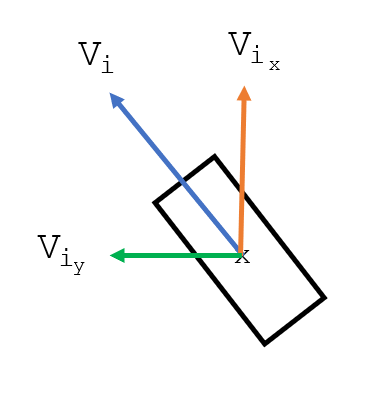
\includegraphics[width=\linewidth]{wheel_vector.png}
        \caption{Vector Definitions}
        \label{fig:vecdef}
      \end{minipage}
      \hfill
      \begin{minipage}[b]{0.45\linewidth}
        \centering
        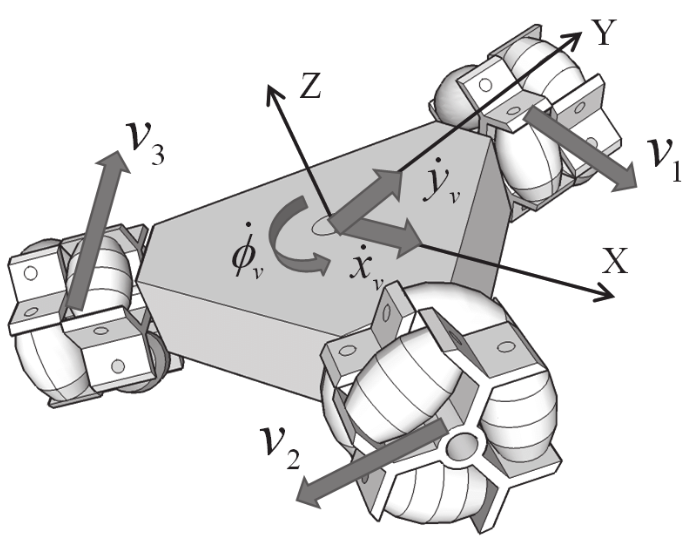
\includegraphics[width=\linewidth]{OWB_vectors.PNG}
        \caption{OWB drive vectors \cite{wada2015OWB}}
        \label{fig:owb_vec}
      \end{minipage}

      \label{fig:vecs}
    \end{figure}

    \newpage

    \section{Double-sided Two Way Ranging}

    \begin{figure}[ht!]
      \begin{center}
          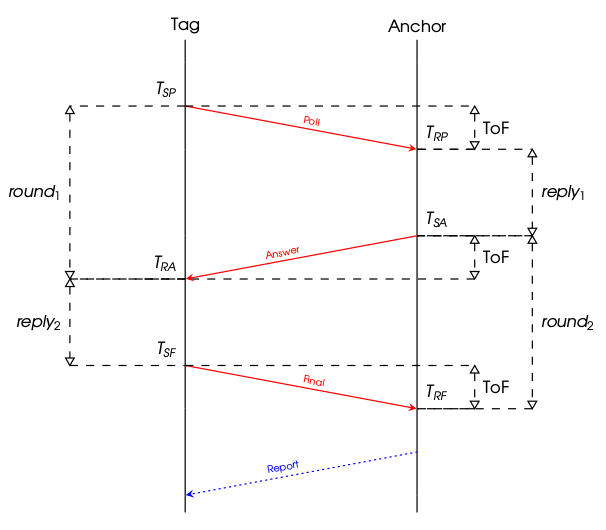
\includegraphics[width=1.0\textwidth]{sds_twr.PNG}\\
          \caption{ Symmetrical Double-sided Two-way Ranging } 
          \label{fig:sds_twr}
      \end{center}
    \end{figure}

    \newpage

    \section{Limit Switch Circuit}

    \begin{figure}[ht!]
      \begin{center}
          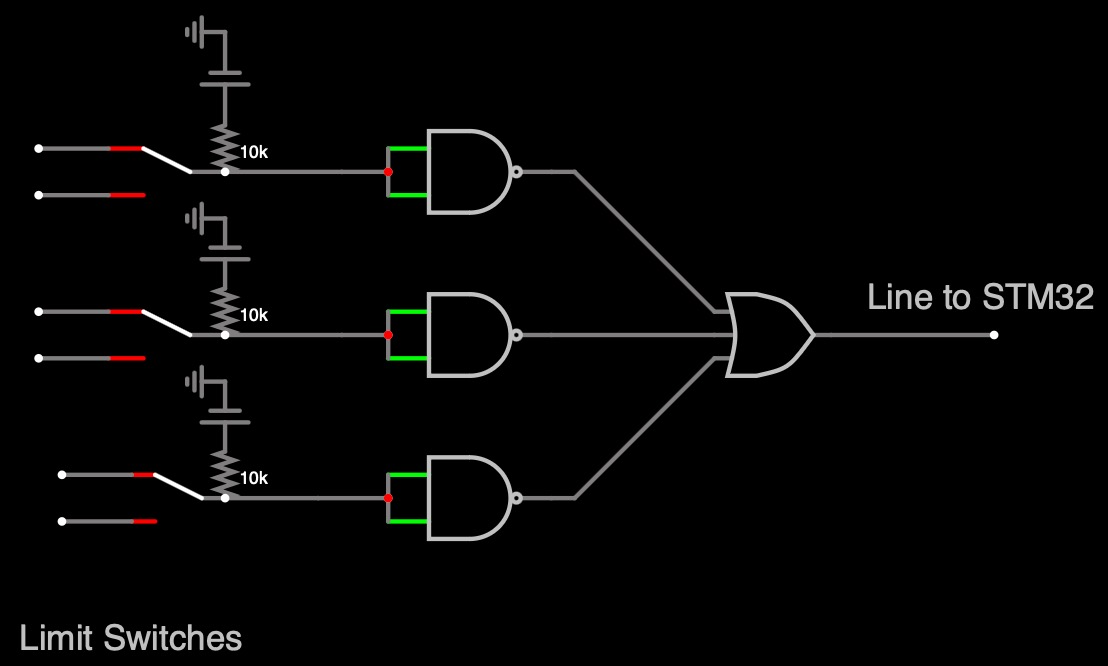
\includegraphics[width=0.6\textwidth]{limitswitchcircuit.png}\\
          \caption{ Limit Switch Circuit } 
          \label{fig:limitswitchcircuit}
      \end{center}
    \end{figure}

    \begin{figure}[ht!]
      \begin{center}
          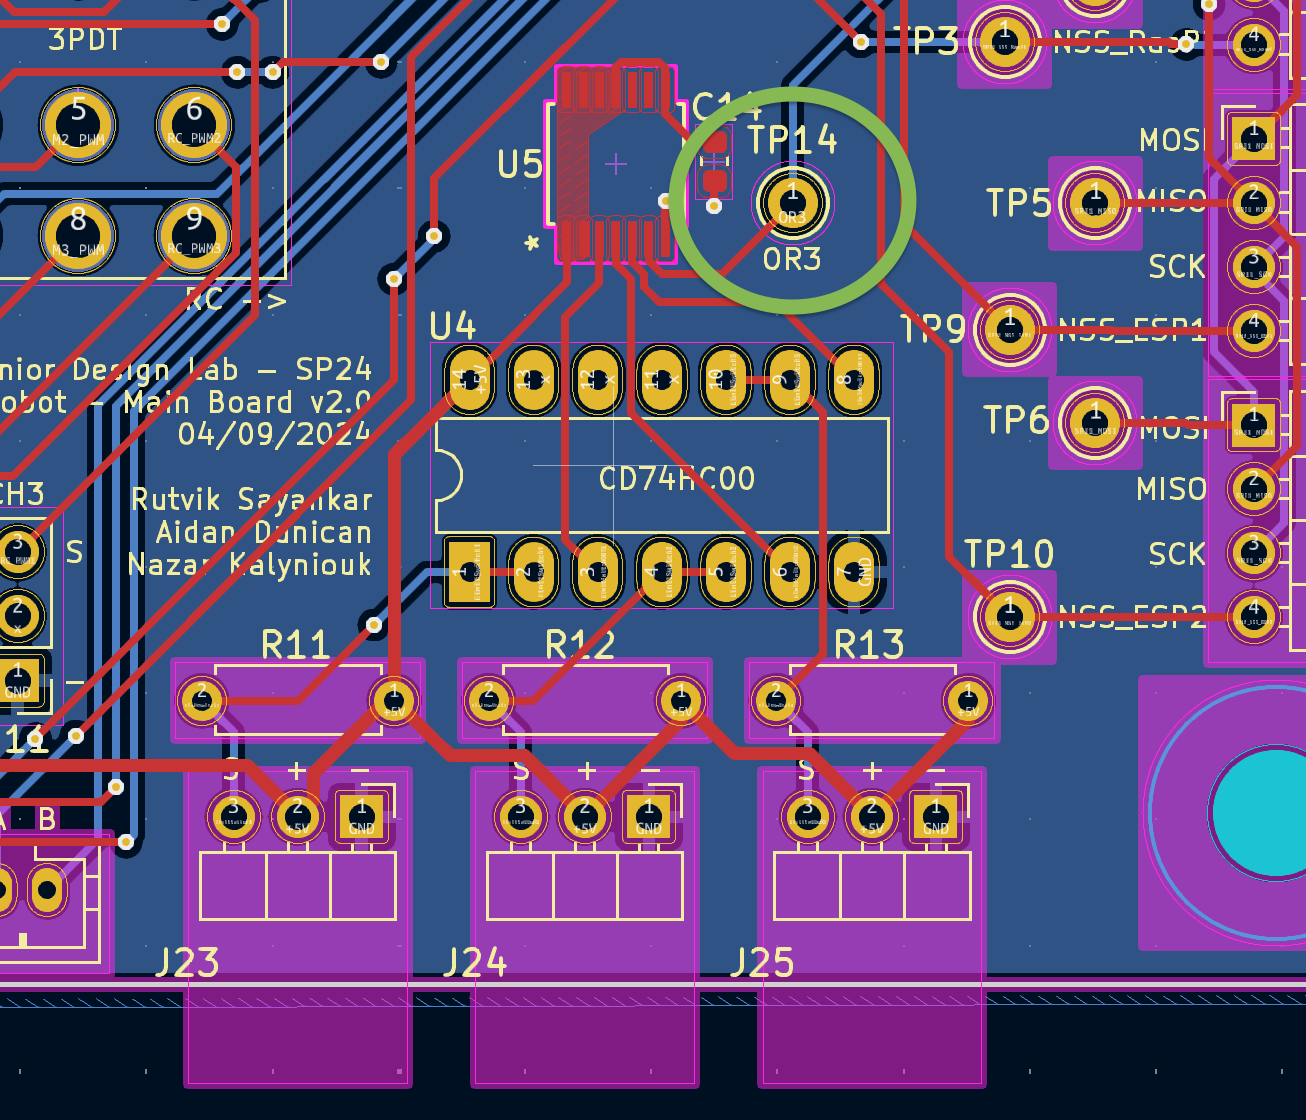
\includegraphics[width=0.8\textwidth]{OR3TestPoint.png}\\
          \caption{ PCB OR3 Test Point } 
          \label{fig:OR3TestPoint}
      \end{center}  
    \end{figure}

    \newpage

    \section{Open CV Images}

    \begin{figure}[ht!]
      \begin{center}
          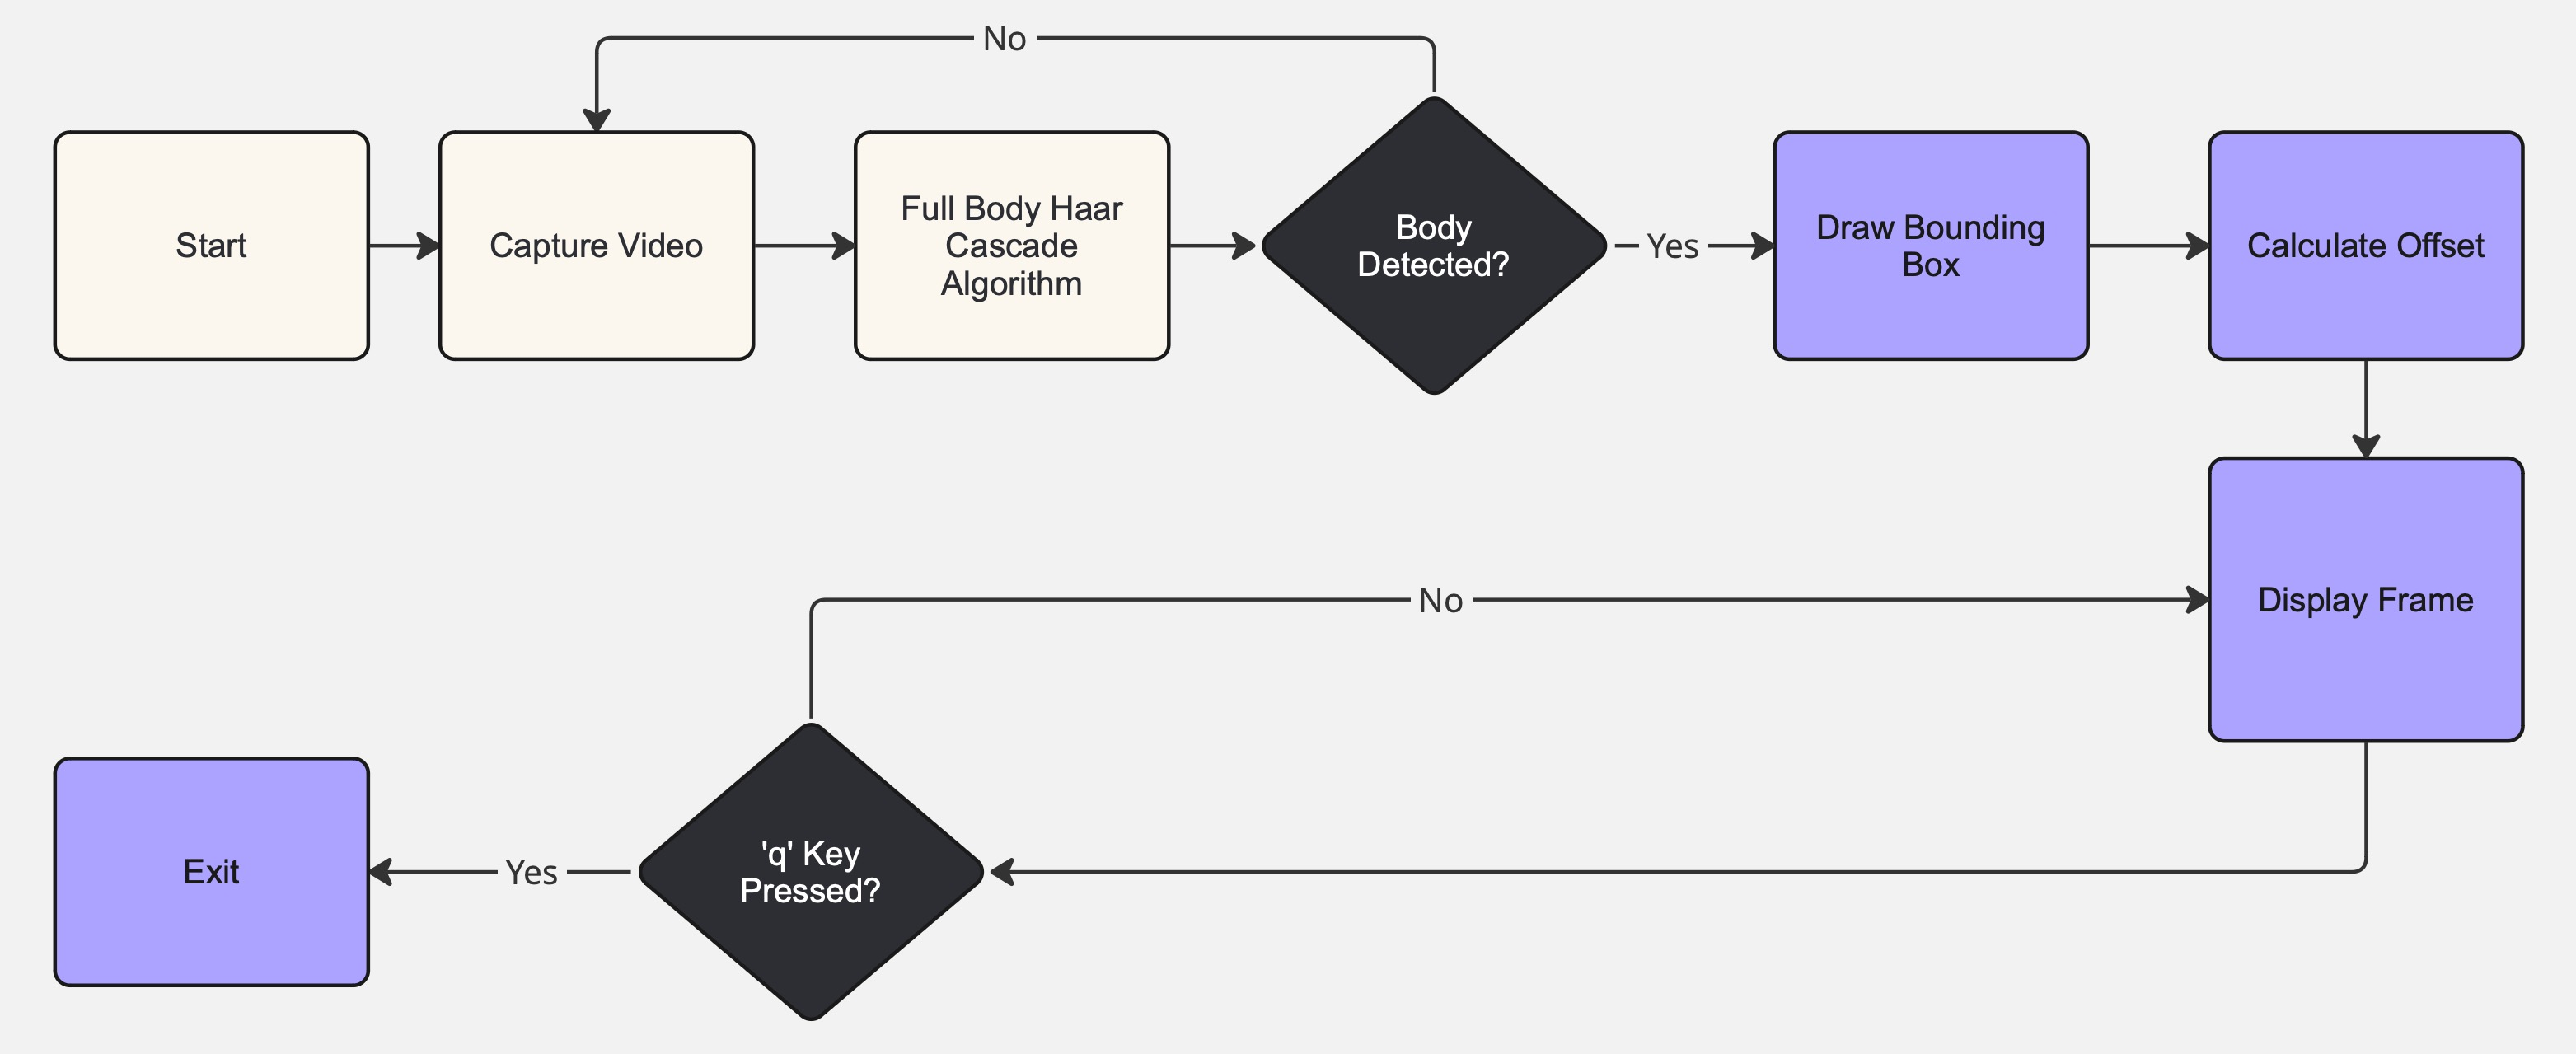
\includegraphics[width=0.8\textwidth]{Flowchart.jpg}\\
          \caption{ OpenCV Algorithm Flowchart  } 
          \label{fig:Flowchart}
      \end{center}
    \end{figure}

    \begin{figure}[ht!]
      \begin{center}
          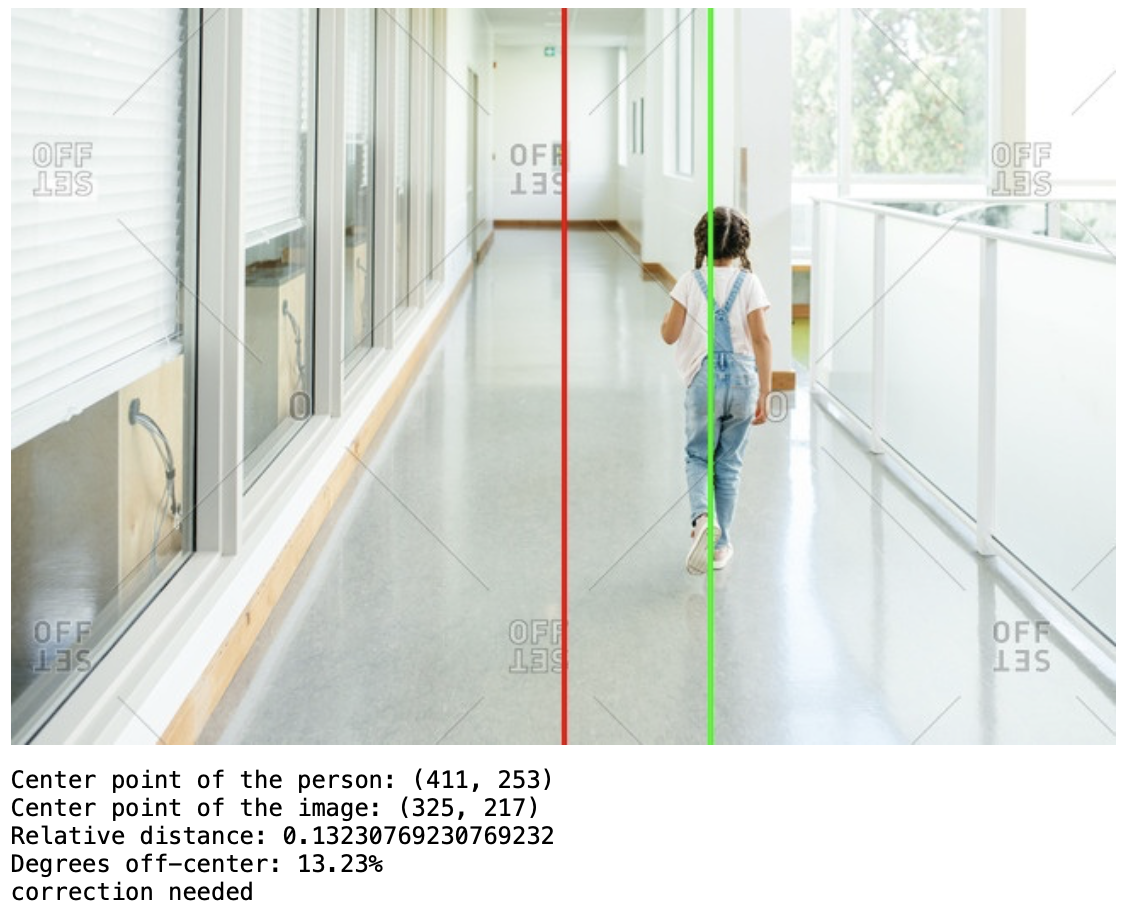
\includegraphics[width=0.6\textwidth]{CVModule_PerformanceTest.png}\\
          \caption{ OpenCV Performance Test } 
          \label{fig:CVModule_PerformanceTest}
      \end{center}
    \end{figure}

    \begin{figure}[ht!]
      \centering
      \begin{minipage}[b]{0.45\linewidth}
        \centering
        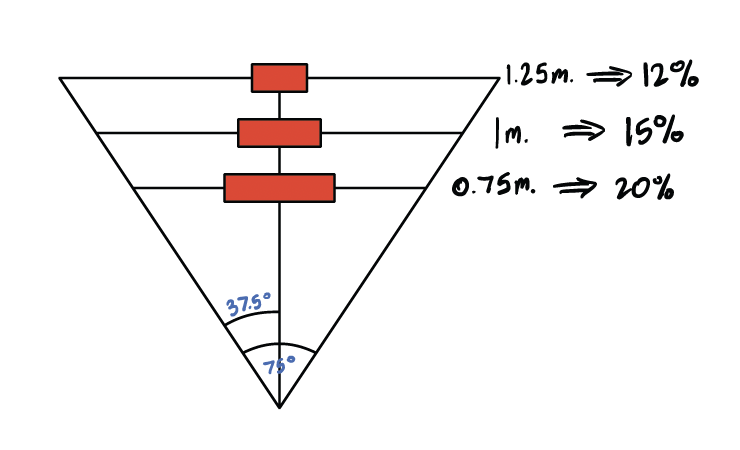
\includegraphics[width=\linewidth]{distance.png}
        \caption{Percent of screen calculations for OpenCV algorithm}
        \label{fig:redboxes}
      \end{minipage}
      \hfill
      \begin{minipage}[b]{0.3\linewidth}
        \centering
        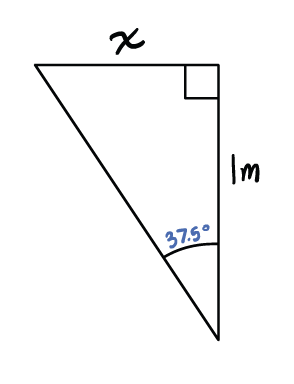
\includegraphics[width=\linewidth]{angle.PNG}
        \caption{Calculation of Horizonatal FOV Width}
        \label{fig:angle}
      \end{minipage}
    \end{figure}

    \newpage

    \section{Power Delivery}

    \begin{figure}[ht!]
      \begin{center}
          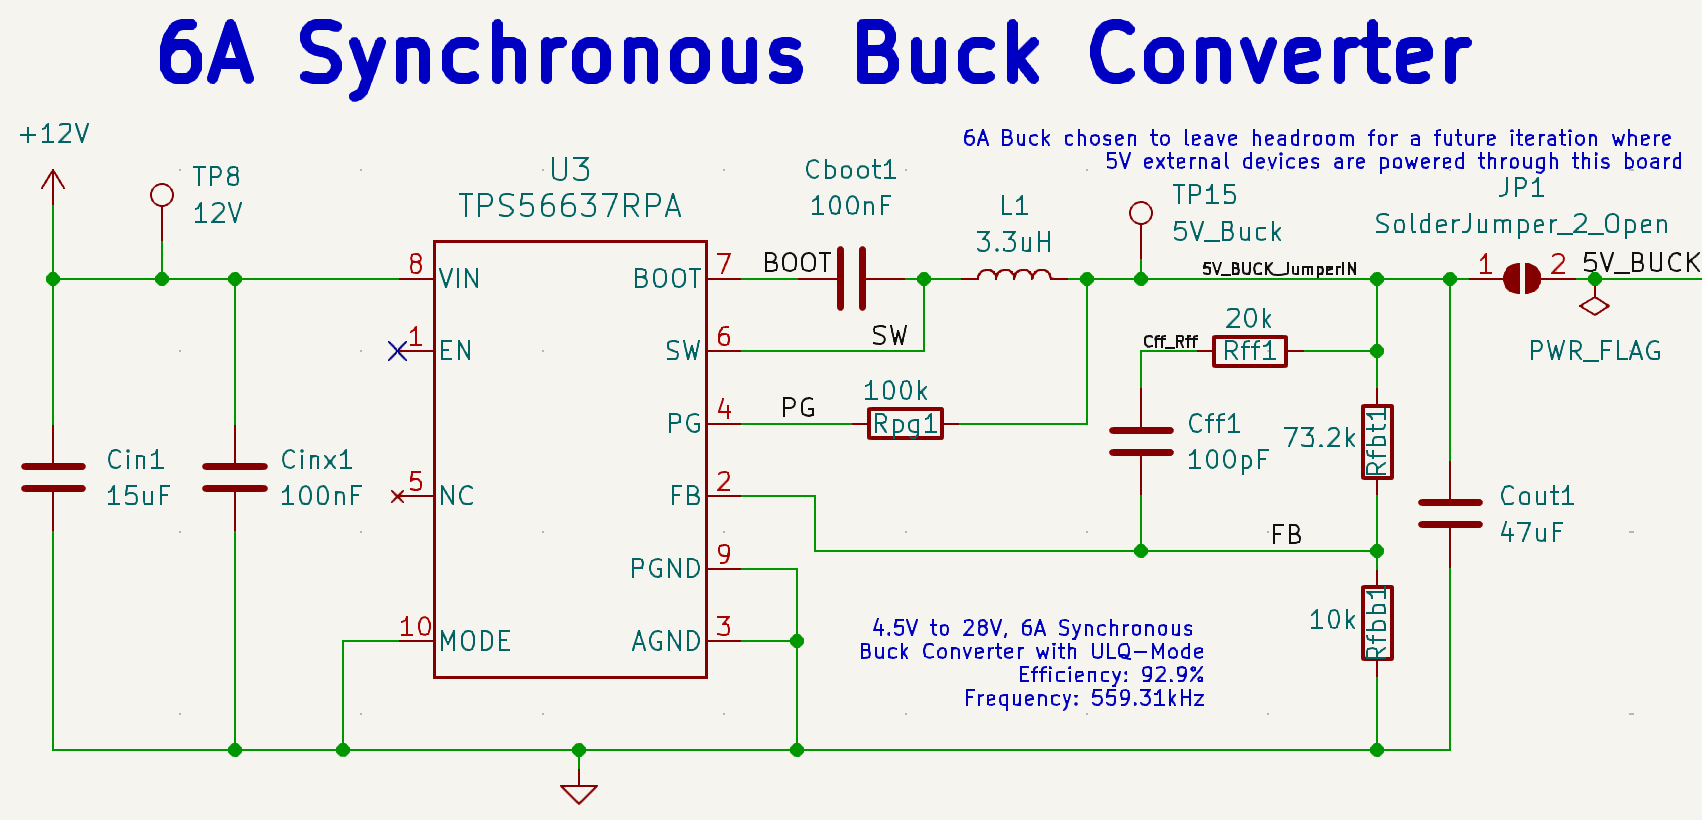
\includegraphics[width=0.8\textwidth]{BuckConverter.png}\\
          \caption{ $5~V$ $6~A$ Buck Converter } 
          \label{fig:BuckConverter}
      \end{center}
    \end{figure}

    \begin{figure}[ht!]
      \begin{center}
          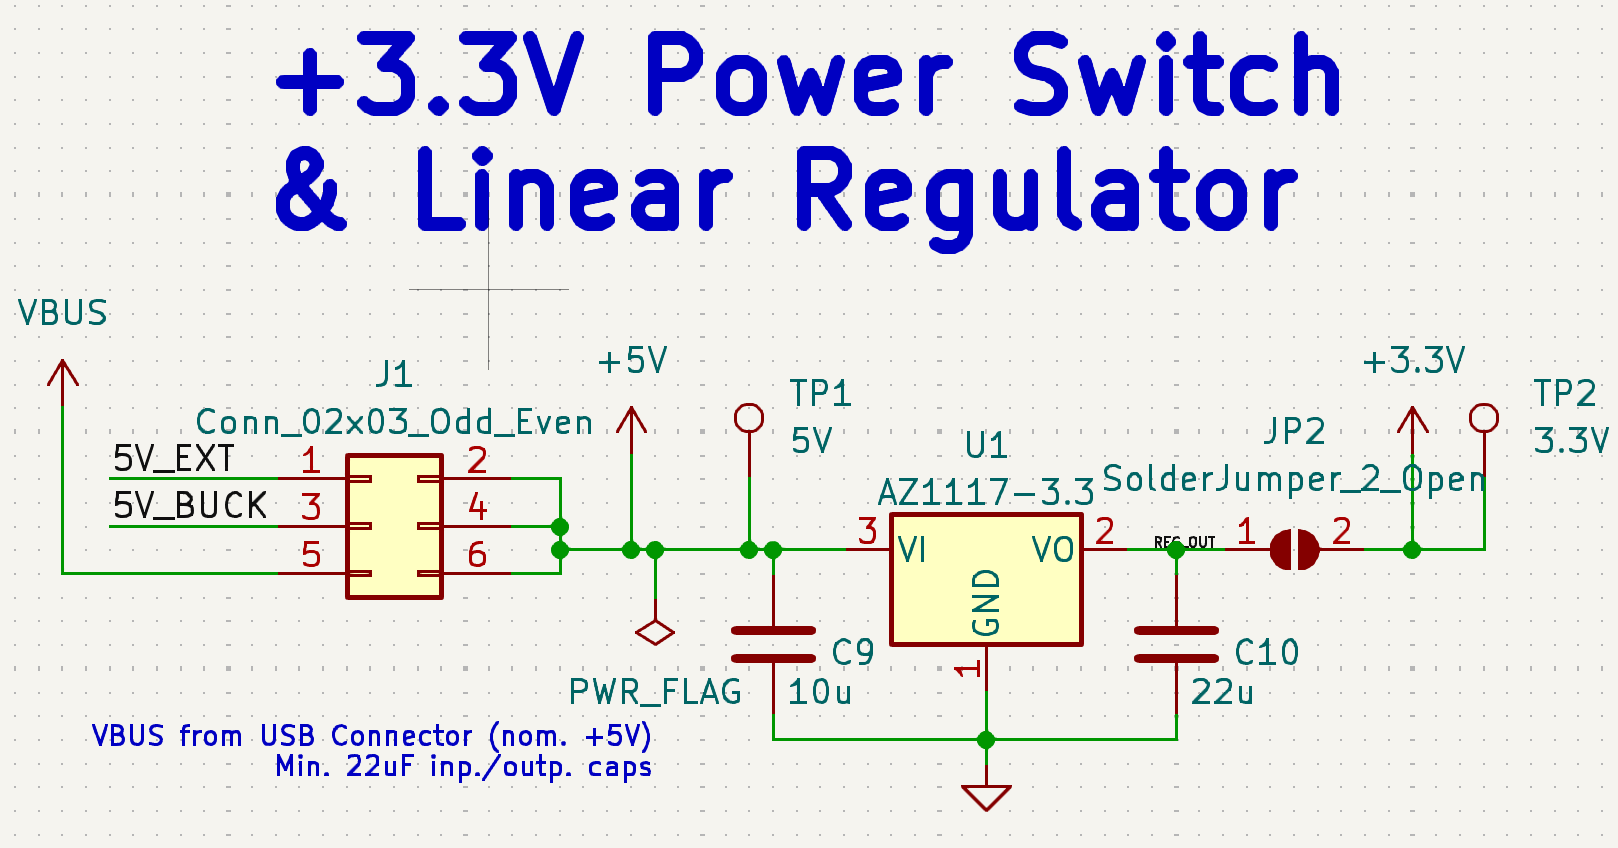
\includegraphics[width=0.8\textwidth]{LDO.png}\\
          \caption{ $3.3~V$ Low Dropout Regulator } 
          \label{fig:LDO}
      \end{center}
    \end{figure}

    \newpage

    \section{UWB Triangulation}

    \begin{figure}[ht!]
      \centering
      \begin{minipage}[b]{0.45\linewidth}
        \centering
        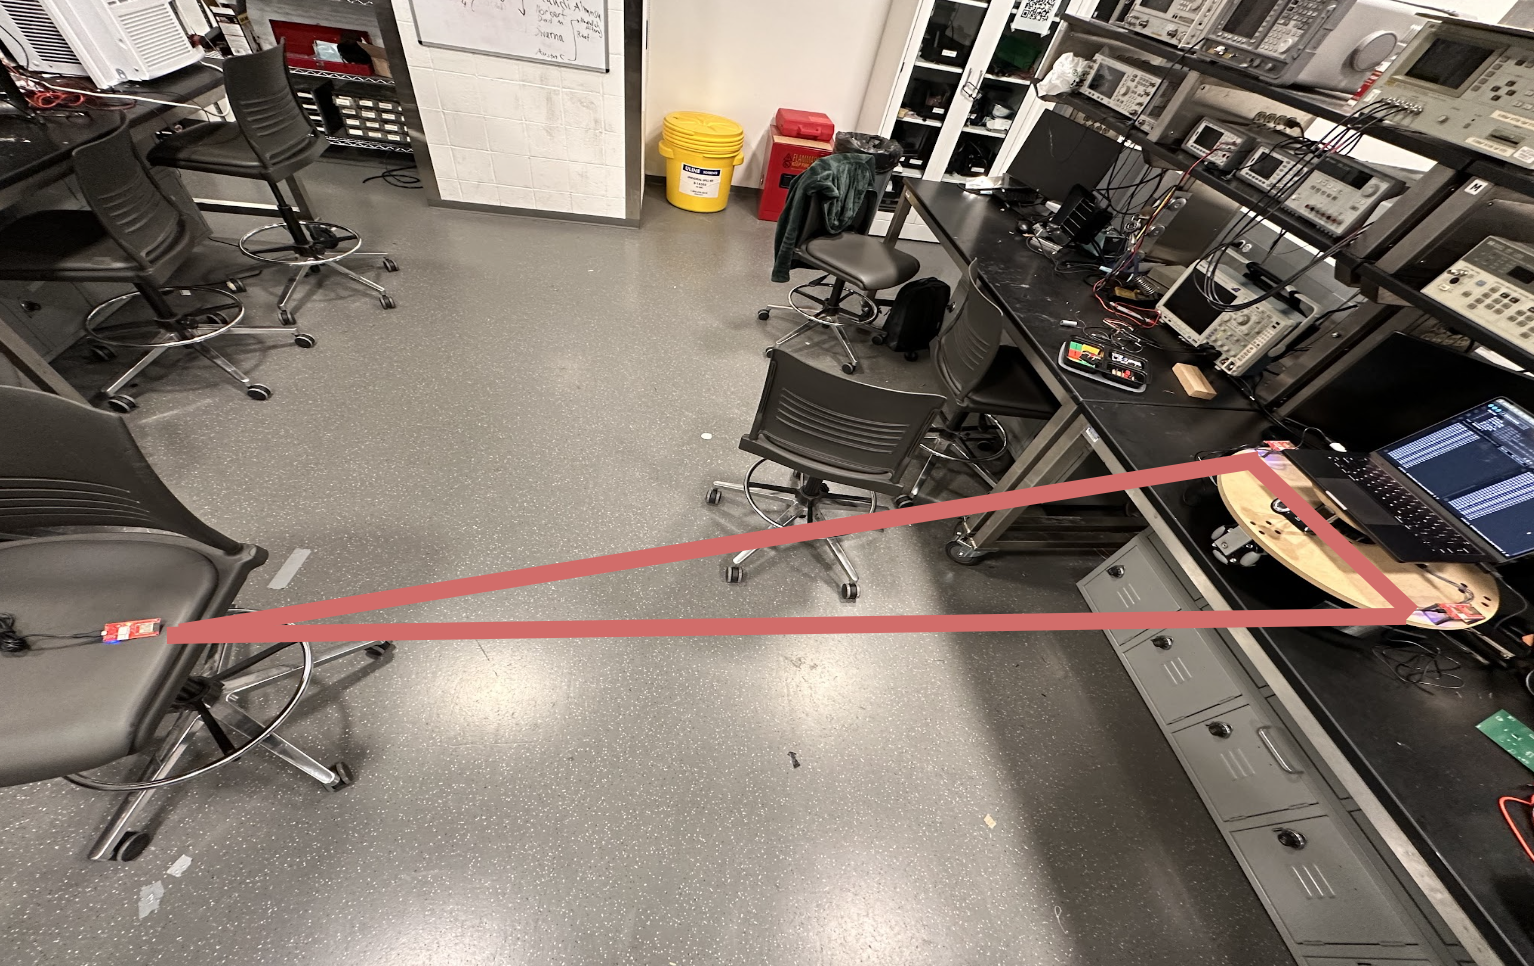
\includegraphics[width=\linewidth]{UWBTriangle.png}
        \caption{UWB Triangle Laid out}
        \label{fig:UWBTriangle}
      \end{minipage}
      \hfill
      \begin{minipage}[b]{0.45\linewidth}
        \centering
        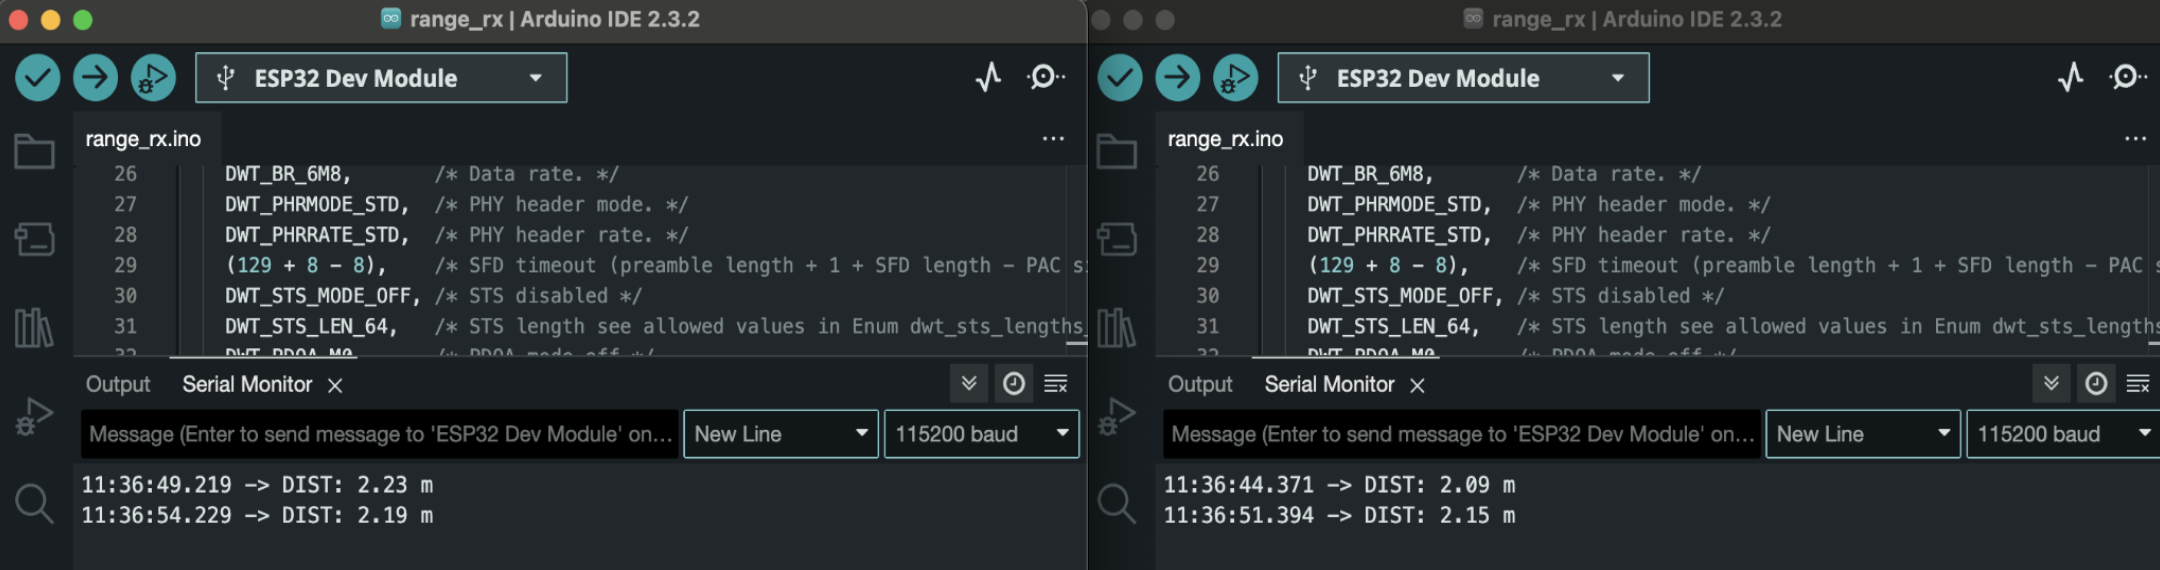
\includegraphics[width=\linewidth]{UWBTriangleSerialOut.PNG}
        \caption{UWB Serial Read Out}
        \label{fig:UWBTriangleSerialOut}
      \end{minipage}
    \end{figure}

    \begin{figure}[ht!]
      \begin{center}
          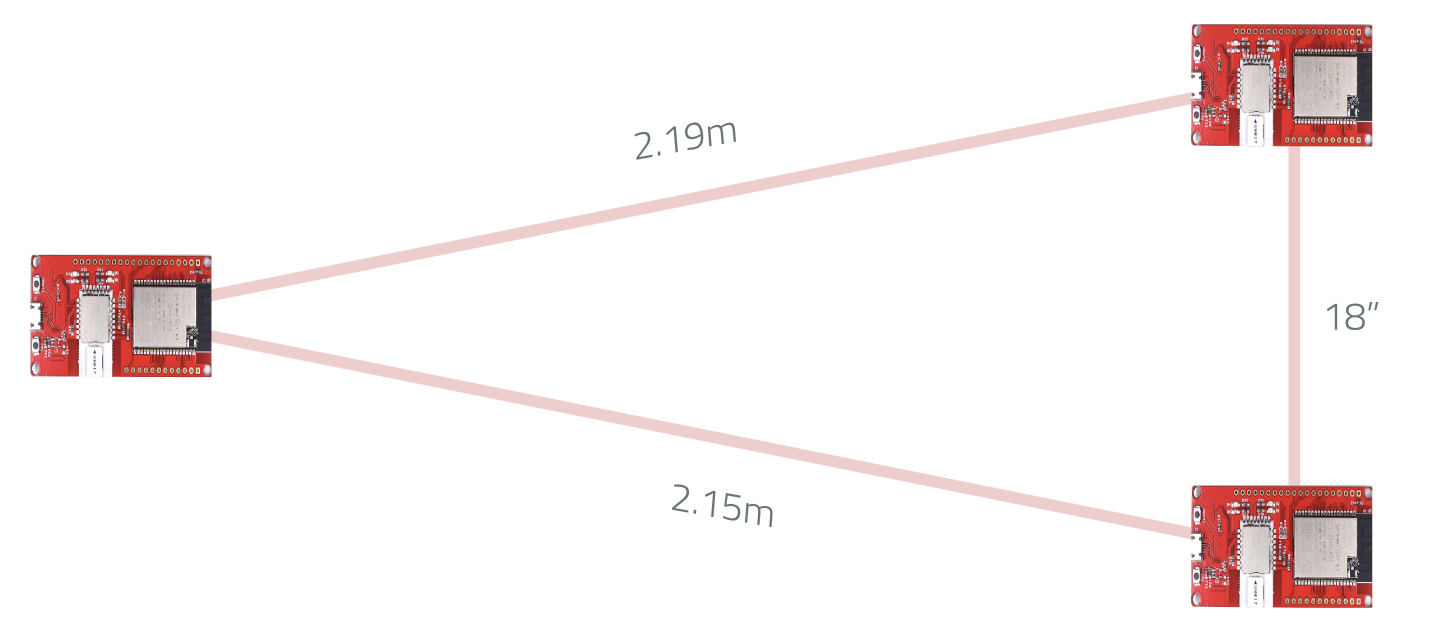
\includegraphics[width=0.6\textwidth]{UWBTriangleFull.png}\\
          \caption{ UWB Triangle with Distances } 
          \label{fig:UWBTriangleFull}
      \end{center}
    \end{figure}

    \begin{figure}[ht!]
      \centering
      \begin{minipage}[b]{0.45\linewidth}
        \centering
        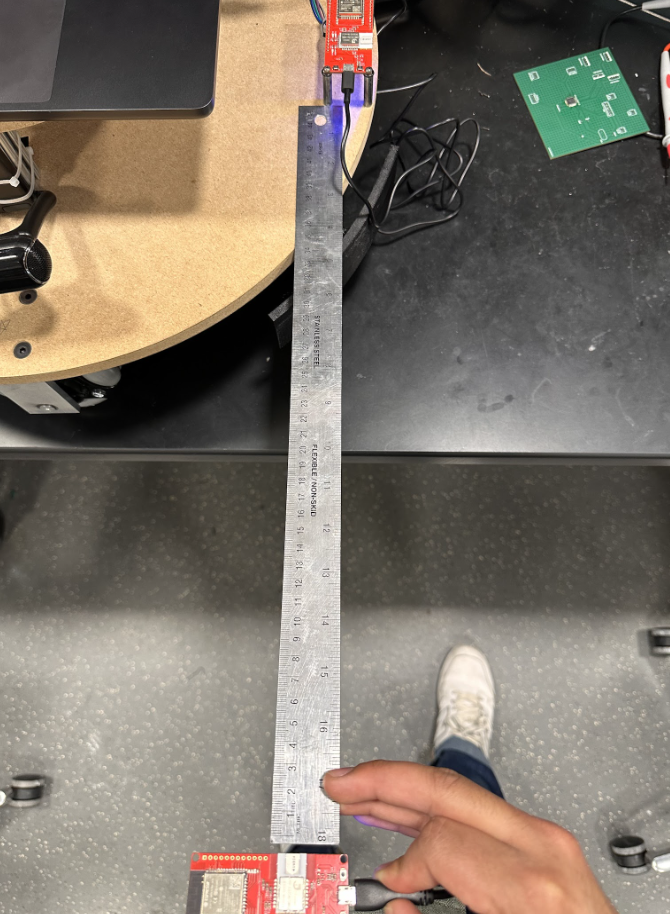
\includegraphics[width=\linewidth]{UWBRuler.png}
        \caption{45" Ruler between UWB Transceiver}
        \label{fig:UWBRuler}
      \end{minipage}
      \hfill
      \begin{minipage}[b]{0.3\linewidth}
        \centering
        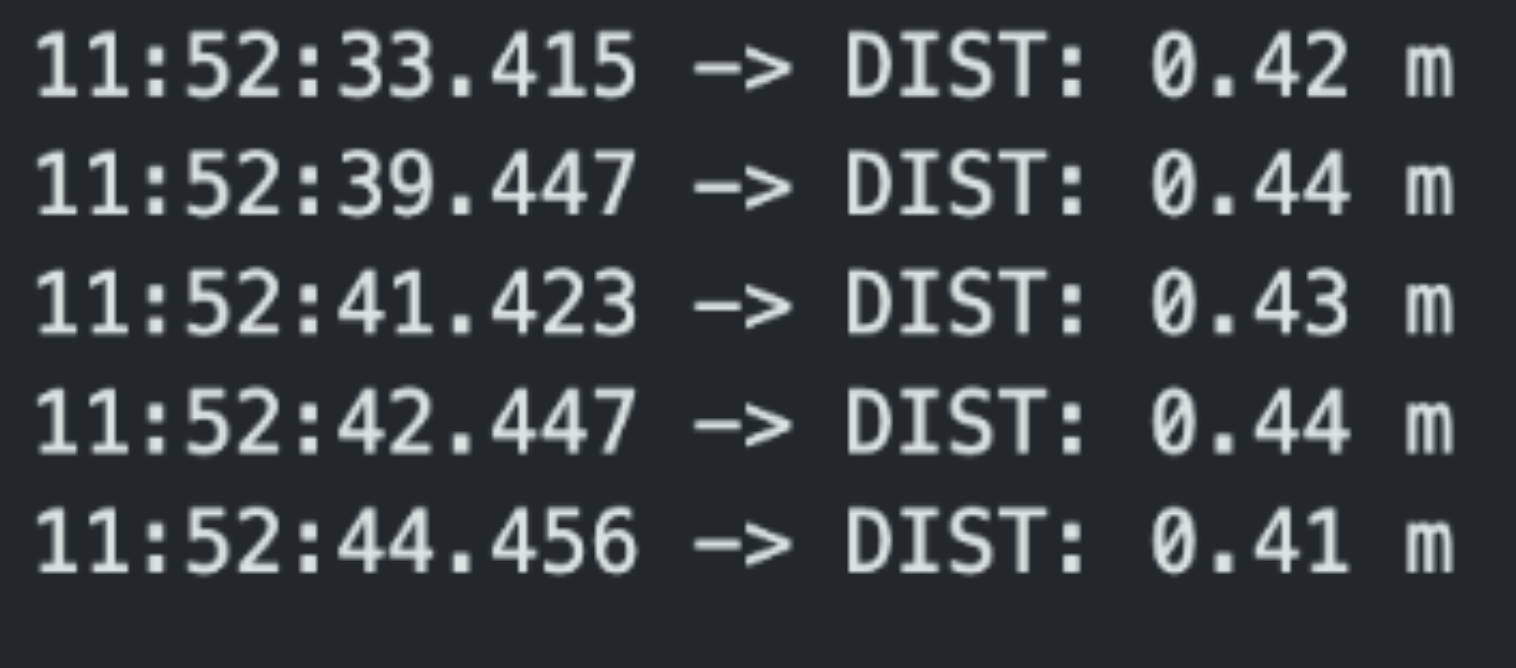
\includegraphics[width=\linewidth]{UWBSerialOut.PNG}
        \caption{UWB Serial Read Out}
        \label{fig:UWBSerialOut}
      \end{minipage}
    \end{figure}

    \newpage

    \section{Computer Vision Verification}

    \begin{figure}[ht!]
      \begin{center}
          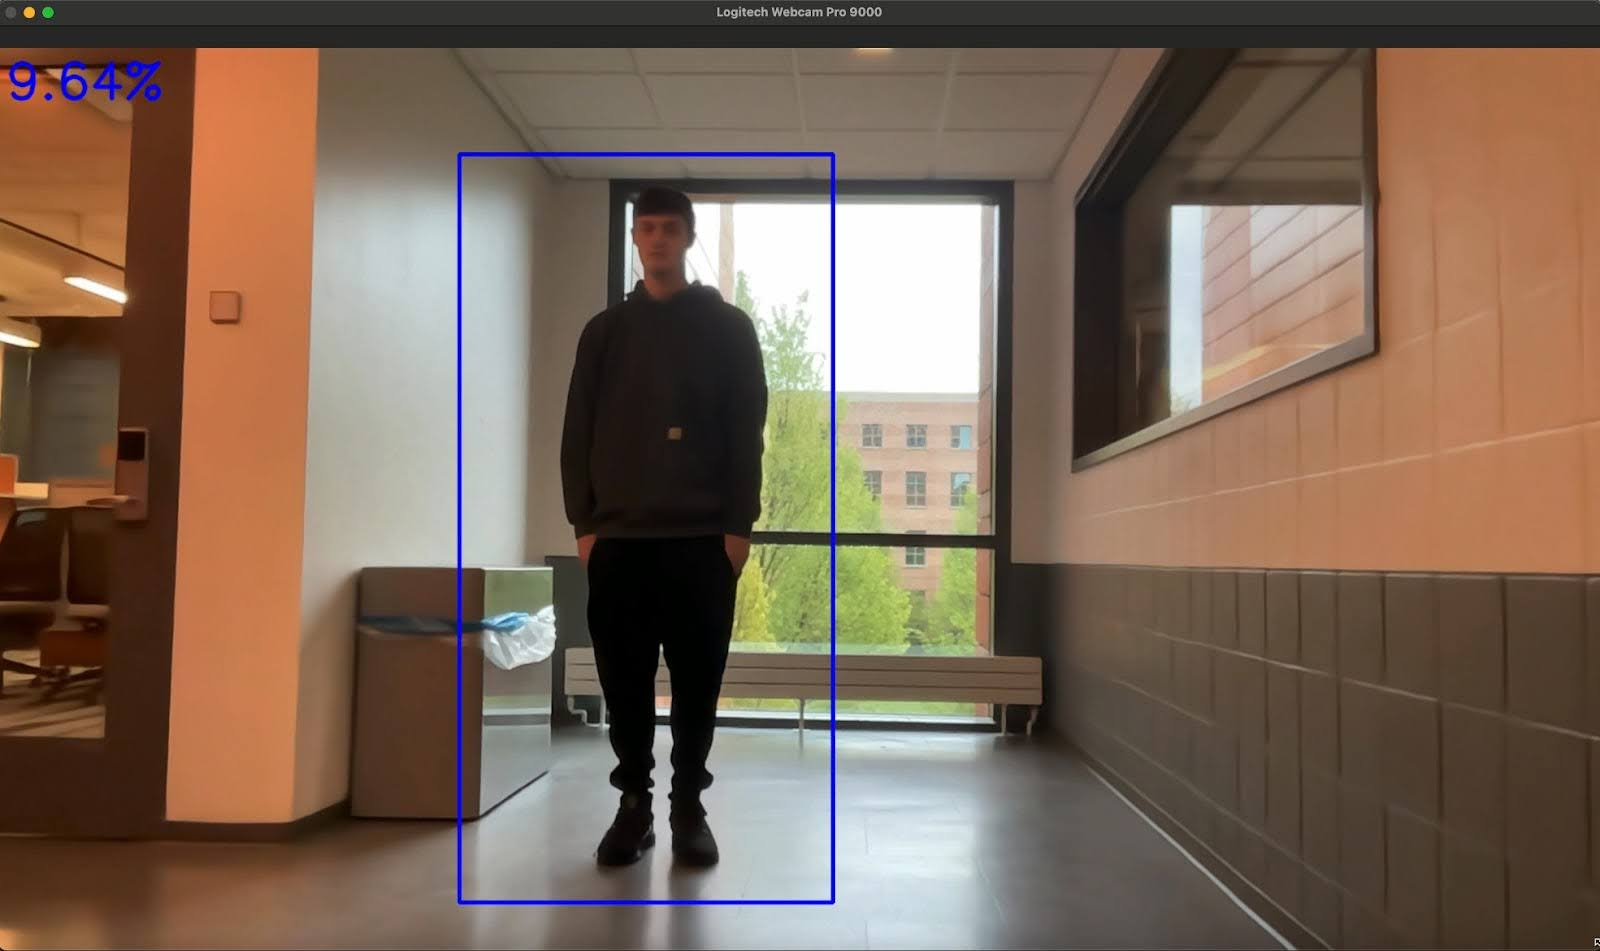
\includegraphics[width=0.8\textwidth]{OpenCVAngle.jpeg}\\
          \caption{ Computer Vision Verification } 
          \label{fig:CVVerification}
      \end{center}  
    \end{figure}

    \newpage

    \section{Control System Verification}

    \begin{figure}[ht!]
      \begin{center}
          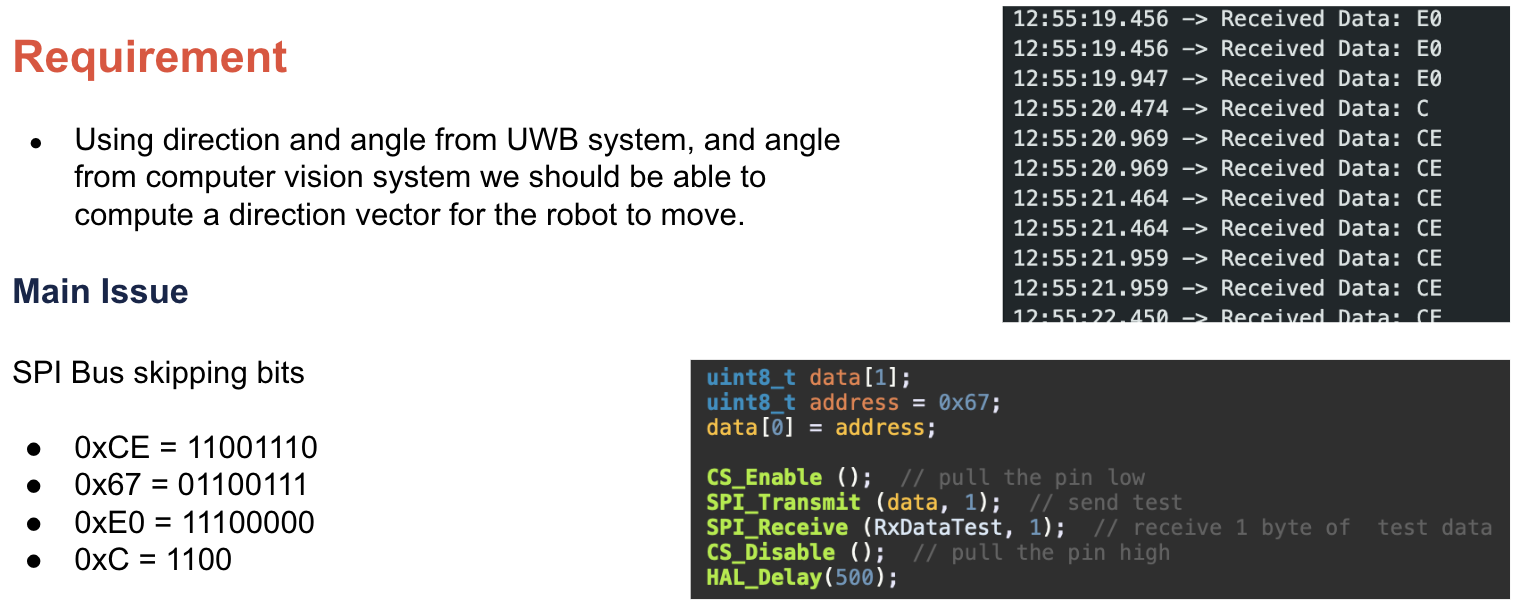
\includegraphics[width=0.9\textwidth]{SPISkipping.png}\\
          \caption{ SPI Bus Skipping Bits } 
          \label{fig:SPISkipping}
      \end{center}  
    \end{figure}

    \newpage

    \section{Power System Verification}

    \begin{figure}[ht!]
      \centering
      \begin{minipage}[b]{0.3\linewidth}
        \centering
        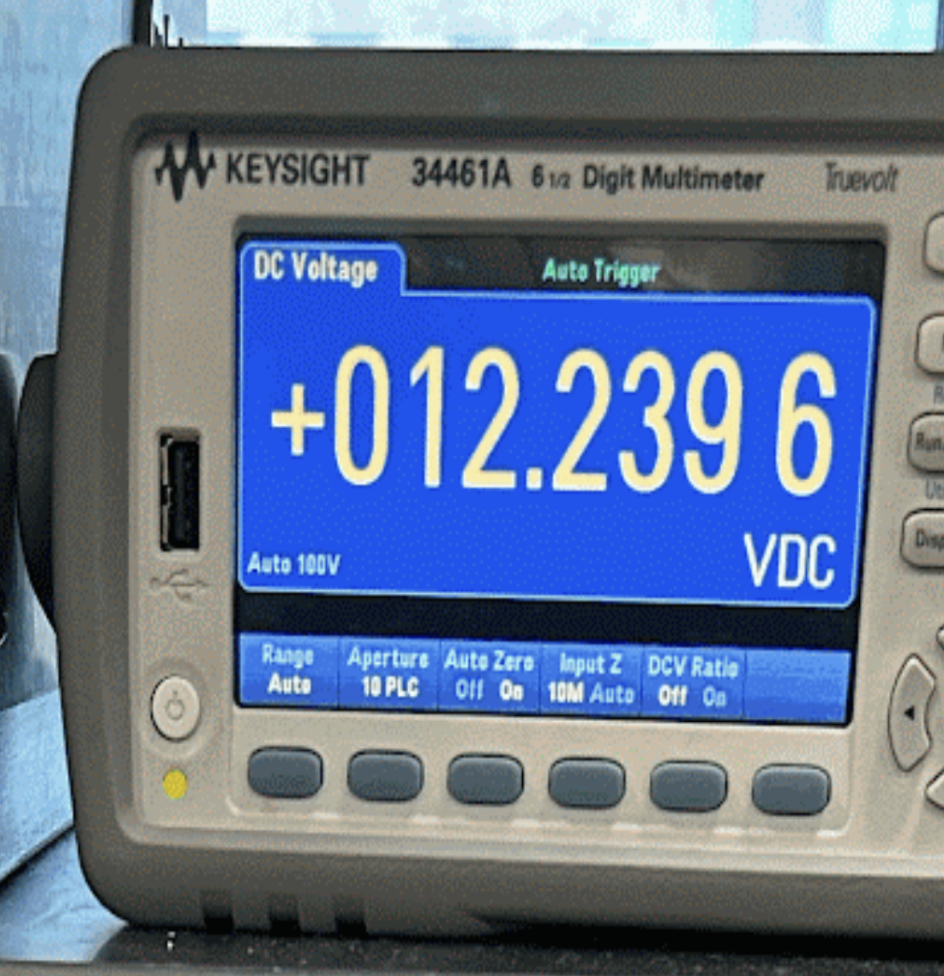
\includegraphics[width=\linewidth]{12VLine.png}
        \caption{$12~V$ Power Line}
        \label{fig:12V}
      \end{minipage}
      \hfill
      \begin{minipage}[b]{0.3\linewidth}
        \centering
        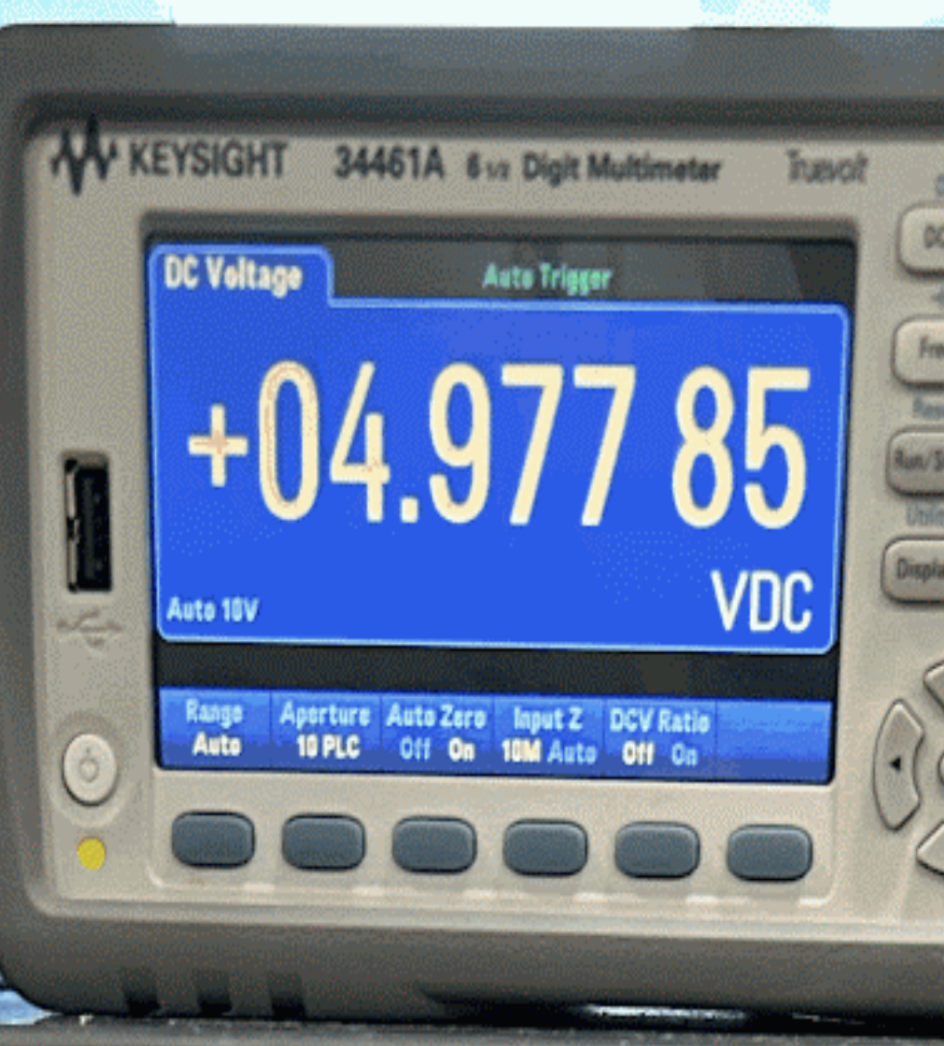
\includegraphics[width=\linewidth]{5VLine.PNG}
        \caption{$5~V$ Power Line}
        \label{fig:5V}
      \end{minipage}
      \hfill
      \begin{minipage}[b]{0.3\linewidth}
        \centering
        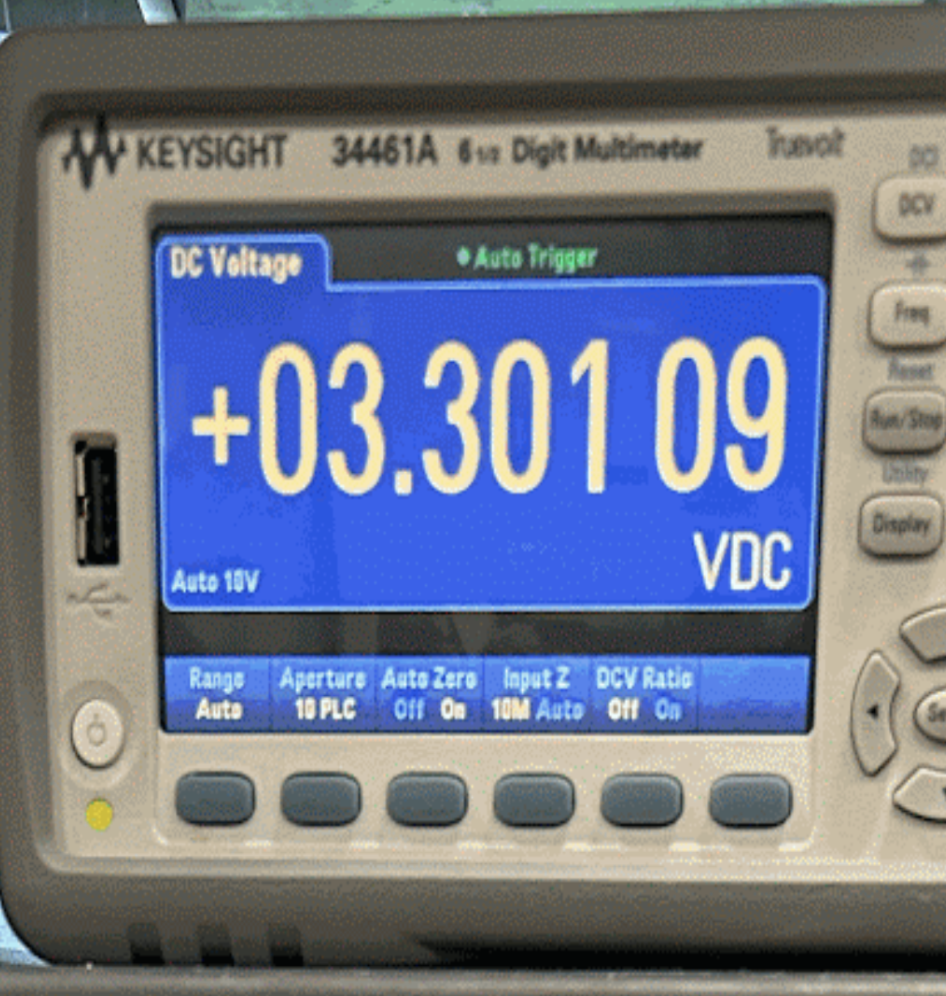
\includegraphics[width=\linewidth]{3VLine.PNG}
        \caption{$3.3~V$ Power Line}
        \label{fig:3V}
      \end{minipage}
    \end{figure}

    \newpage

    \section{RC Controller}
    \begin{figure}[ht!]
      \begin{center}
          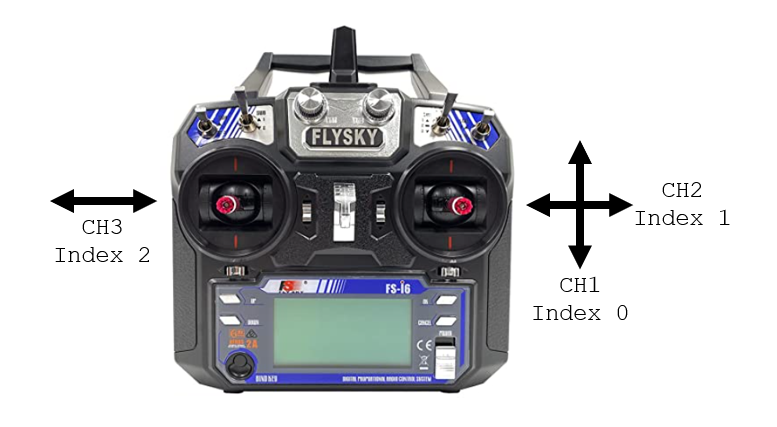
\includegraphics[width=1.0\textwidth]{channel.PNG}\\
          \caption{ Channel Distribution  } 
          \label{fig:RCController}
      \end{center}
    \end{figure}

    \newpage

    \section{STM32 Pinout}

    \begin{figure}[ht!]
      \begin{center}
          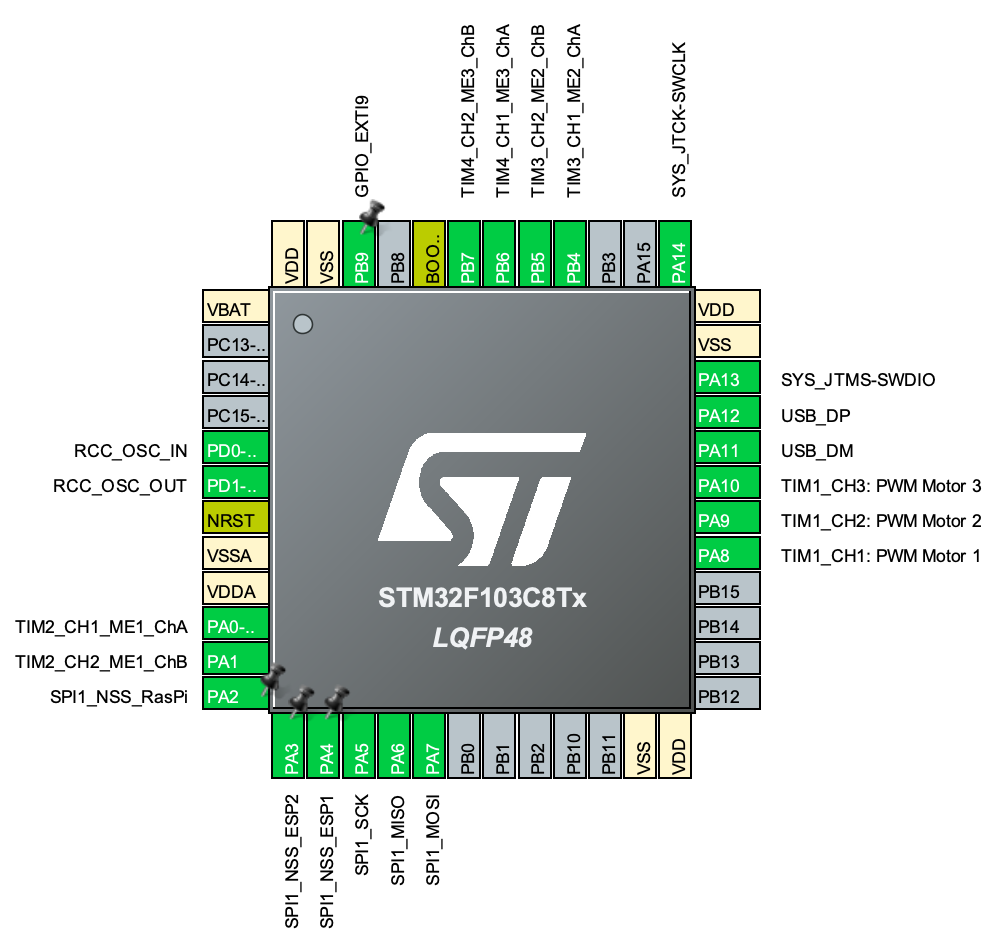
\includegraphics[width=1.0\textwidth]{STM32Pinout.PNG}\\
          \caption{ STM32F103C8T6 Pinout } 
          \label{fig:STM32Pinout}
      \end{center}
    \end{figure}

    \newpage

    \section{STM32 Code}

    \begin{figure}
      \begin{lstlisting}[language=C]
        void HAL_GPIO_EXTI_Callback(uint16_t GPIO_Pin) {
          if((GPIO_Pin == GPIO_PIN_9)) {
            if((HAL_GPIO_ReadPin(GPIOB, GPIO_PIN_9) == GPIO_PIN_SET)){
                HAL_TIM_PWM_Stop(&htim1, TIM_CHANNEL_1);
                HAL_TIM_PWM_Stop(&htim1, TIM_CHANNEL_2);
                HAL_TIM_PWM_Stop(&htim1, TIM_CHANNEL_3);
                }
          }
          else{
            __NOP();
          }
        }
        \end{lstlisting}
        \caption{Limit Switch Interrupt Functionality}
        \label{fig:interrupt}
    \end{figure}

    \begin{figure}
      \begin{lstlisting}[language=C]
        void SPIConfig (void){
          RCC->APB2ENR |= (1<<12);  // Enable SPI1 CLock
          SPI1->CR1 |= (1<<0)|(1<<1);   // CPOL=1, CPHA=1
          SPI1->CR1 |= (1<<2);  // Master Mode
          SPI1->CR1 |= (3<<3);  // BR[2:0] = 011: fPCLK/16, PCLK2 = 80MHz, SPI clk = 5MHz
          SPI1->CR1 &= ~(1<<7);  // LSBFIRST = 0, MSB first
          SPI1->CR1 |= (1<<8) | (1<<9);  // SSM=1, SSi=1 -> Software Slave Management
          SPI1->CR1 &= ~(1<<10);  // RXONLY = 0, full-duplex
          SPI1->CR1 &= ~(1<<11);  // DFF=0, 8 bit data
          SPI1->CR2 = 0;
        }
	    \end{lstlisting}
     \caption{SPI Config Setup}
     \label{fig:SPIConfig}
    \end{figure}

    \newpage

    \begin{figure}
      \begin{lstlisting}[language=C]
        void SPI_Transmit (uint8_t *data, int size){

          /************** STEPS *****************
          1. Wait for the TXE bit to set in the Status Register
          2. Write the data to the Data Register
          3. After the data has been transmitted, wait for the BSY bit to reset in Status Register
          4. Clear the Overrun flag by reading DR and SR
          ************************************************/

          int i=0;
          while (i<size){
            while (!((SPI1->SR)&(1<<1))) {};  // wait for TXE bit to set -> This will indicate that the buffer is empty
            SPI1->DR = data[i];  // load the data into the Data Register
            i++;
          }

        /*During discontinuous communications, there is a 2 APB clock period delay between the
        write operation to the SPI_DR register and BSY bit setting. As a consequence it is
        mandatory to wait first until TXE is set and then until BSY is cleared after writing the last
        data.
        */
          while (!((SPI1->SR)&(1<<1))) {};  // wait for TXE bit to set -> This will indicate that the buffer is empty
          while (((SPI1->SR)&(1<<7))) {};  // wait for BSY bit to Reset -> This will indicate that SPI is not busy in communication

          //  Clear the Overrun flag by reading DR and SR
          uint8_t temp = SPI1->DR;
                  temp = SPI1->SR;
        }
      \end{lstlisting}
      \caption{SPI Transmit Setup}
      \label{fig:SPI_Transmit}
    \end{figure}

\begin{figure}
      \begin{lstlisting}[language=C]
        void SPI_Receive (uint8_t *data, int size){
          /************** STEPS *****************
          1. Wait for the BSY bit to reset in Status Register
          2. Send some Dummy data before reading the DATA
          3. Wait for the RXNE bit to Set in the status Register
          4. Read data from Data Register
          ************************************************/

          while (size){
            while (((SPI1->SR)&(1<<7))) {};  // wait for BSY bit to Reset -> This will indicate that SPI is not busy in communication
            SPI1->DR = 0;  // send dummy data
            while (!((SPI1->SR) &(1<<0))){};  // Wait for RXNE to set -> This will indicate that the Rx buffer is not empty
            *data++ = (SPI1->DR);
            size--;
          }
        }
      \end{lstlisting}
      \caption{SPI Receive Setup}
      \label{fig:SPI_Receive}
    \end{figure}

\begin{figure}
      \begin{lstlisting}[language=C]
        void GPIOConfig (void){
          RCC->APB2ENR |=  (1<<2);  // Enable GPIOA clock
          GPIOA->CRL = 0;
          GPIOA->CRL |= (11U<<20);   // PA5 (SCK) AF output Push Pull
          GPIOA->CRL |= (11U<<28);   // PA7 (MOSI) AF output Push Pull
          GPIOA->CRL |= (1<<26);    // PA6 (MISO) Input mode (floating)
          GPIOA->CRL |= (3<<16);    // PA4 used for CS, GPIO Output
        }
	    \end{lstlisting}
    \caption{SPI GPIO Chip Select Setup}
    \label{fig:GPIOConfig}
\end{figure}

\begin{figure}
      \begin{lstlisting}[language=C]
        void SPI_Enable (void){
          SPI1->CR1 |= (1<<6);   // SPE=1, Peripheral enabled
        }

        void SPI_Disable (void){
          SPI1->CR1 &= ~(1<<6);   // SPE=0, Peripheral Disabled
        }

        void CS_Enable (void){
          GPIOA->BSRR |= (1<<9)<<16;
        }

        void CS_Disable (void){
          GPIOA->BSRR |= (1<<9);
        }

        uint8_t RxData[3]; // receive SPI data bytes
        
        \end{lstlisting}
        \caption{SPI Enable and Disable Setup}
        \label{fig:SPI_Enable}
    \end{figure}

    \begin{figure}
      \begin{lstlisting}[language=C]
        // Maps PWM speed between a range
        uint32_t MAP(uint32_t au32_IN, uint32_t au32_INmin, uint32_t au32_INmax, uint32_t au32_OUTmin, uint32_t au32_OUTmax){
            return ((((au32_IN - au32_INmin)*(au32_OUTmax - au32_OUTmin))/(au32_INmax - au32_INmin)) + au32_OUTmin);
        }
        
        // Maps speed between a limit
        int mapChannel(int speed, int minLimit, int maxLimit){
          return MAP(speed, -20, 20, minLimit, maxLimit);
        }

        // PWM Timer Setup
        MX_TIM1_Init(); // Initialize all configured peripherals

        HAL_TIM_PWM_Start(&htim1, TIM_CHANNEL_1); // Setting up PWM Timer
        HAL_TIM_PWM_Start(&htim1, TIM_CHANNEL_2); // Setting up PWM Timer
        HAL_TIM_PWM_Start(&htim1, TIM_CHANNEL_3); // Setting up PWM Timer

        HAL_TIM_Encoder_Start_IT(&htim2, TIM_CHANNEL_ALL); // Setting up Encoders
        HAL_TIM_Encoder_Start_IT(&htim3, TIM_CHANNEL_ALL);
        HAL_TIM_Encoder_Start_IT(&htim4, TIM_CHANNEL_ALL);

        while(1){
          htim1.Instance->CCR1 = mapChannel(M1_Speed, 1100, 1884); // current, minimum, maximum, default
          htim1.Instance->CCR2 = mapChannel(M2_Speed, 1100, 1884);
          htim1.Instance->CCR3 = mapChannel(M3_Speed, 1100, 1884);

          HAL_Delay(3000);
        }

	    \end{lstlisting}
     \caption{PWM Setup and Motor Control}
     \label{fig:PWM}
    \end{figure}


    \appendix

    \chapter{Appendix}

    \section{Terms and Keywords}
    \begin{itemize}
        \item ChILD - Children's Interstitial and Diffuse Lung Disease
        \item PCB – Printed Circuit Board
        \item OWB - Three-Wheeled Omni-Wheel Bot
        \item UWB - Ultra-wideband is a radio technology that can use a very low energy level for short-range, high-bandwidth communications over a large portion of the radio spectrum.
        \item ESP32 - A series of low-cost, low-power system-on-a-chip microcontrollers with integrated Wi-Fi and dual-mode Bluetooth.
        \item RPM - Revolutions per minute
        \item GPIO - General-purpose input/output
        \item SPI - Serial Peripheral Interface
        \item PWM - Pulse-width modulation
        \item MPH - Miles per hour
        \item OpenCV - (Open Source Computer Vision Library) is an open source computer vision and machine learning software library.
        \item TDoA - Time Difference of Arrival 
        \item ToF - Time of Flight
        \item BOM - Bill of materials
        \item BLE - Bluetooth Low Energy
        \item LDO - Low Dropout Voltage Regulator
        \item PTC - Positive Temperature Coefficient, PTC fuses are made of a material that increases its internal resistance as the temperature increases.
    \end{itemize}

    \bibliographystyle{IEEEtran}
    \bibliography{ref}

\end{document} % This is the end of the document